% Generated fragments require trusted human review before compilation.
% This binder never requests shell escape or runs external tools.
\documentclass[11pt]{article}
% Trusted shared apparatus. Requires LuaLaTeX; never use shell escape.
\usepackage{fontspec}
\defaultfontfeatures{Ligatures=TeX}
\IfFontExistsTF{Noto Serif}{\setmainfont{Noto Serif}}{%
  \IfFontExistsTF{DejaVu Serif}{\setmainfont{DejaVu Serif}}{%
    \IfFontExistsTF{Times New Roman}{\setmainfont{Times New Roman}}{%
      \PackageError{gelfand-binder}{No configured Cyrillic serif font installed}{Install Noto Serif or DejaVu Serif, or select an installed Cyrillic font.}%
    }%
  }%
}
\IfFontExistsTF{Noto Sans}{\setsansfont{Noto Sans}}{%
  \IfFontExistsTF{DejaVu Sans}{\setsansfont{DejaVu Sans}}{\setsansfont{Arial}}%
}
\IfFontExistsTF{Noto Sans Mono}{\setmonofont{Noto Sans Mono}}{%
  \IfFontExistsTF{DejaVu Sans Mono}{\setmonofont{DejaVu Sans Mono}}{\setmonofont{Courier New}}%
}
\usepackage[a4paper,margin=22mm]{geometry}
\usepackage{amsmath,amssymb,amsthm,mathtools}
\usepackage{xcolor}
\usepackage{tikz}
\usepackage{tikz-cd}
\usetikzlibrary{arrows.meta,positioning,calc}
\usepackage{hyperref}
\hypersetup{unicode=true,colorlinks=true,linkcolor=blue,pdftitle={Gelfand transcription binder}}
\newtheorem{theorem}{Theorem}
\newtheorem{lemma}{Lemma}
\newtheorem{proposition}{Proposition}
\newtheorem{corollary}{Corollary}
\theoremstyle{definition}
\newtheorem{definition}{Definition}
\newtheorem{example}{Example}
\theoremstyle{remark}
\newtheorem{remark}{Remark}
\setlength{\parindent}{0pt}
\setlength{\parskip}{0.55em}
\setlength{\emergencystretch}{3em}
\newcommand{\SourcePage}[2]{%
  \clearpage\phantomsection\label{#1:source-page}%
  \addcontentsline{toc}{subsection}{#1}%
  {\small\sffamily\color{blue!60!black}Source scan frame: #1; visible page/leaf label: #2}\par\medskip%
}
\newcommand{\Unclear}[3]{%
  \begingroup\color{orange!70!black}%
  [Unresolved reading #1/#2: #3]\endgroup%
}
\newcommand{\Incomplete}[3]{%
  \par\begingroup\color{red!65!black}\textbf{Incomplete #1/#2:} #3\endgroup\par%
}
\newcommand{\SourceFigure}[3]{%
  \par\begingroup\color{blue!60!black}\textbf{\hyperref[#1:source-page]{Source figure #1/#2}:} #3%
  \par\textit{Consult the authoritative scan at this locator.}\endgroup\par%
}



% Reader layout only. Original diplomatic text is retained verbatim.
\setlength{\parskip}{0.35em}
\setlength{\emergencystretch}{4em}
\renewcommand{\SourcePage}[2]{%
  \par\addvspace{1em}\phantomsection\label{#1:source-page}%
  \addcontentsline{toc}{subsection}{#1}%
  {\footnotesize\sffamily\color{blue!55!black}#1%
    \def\givenlabel{#2}\def\nolabel{unlabelled}%
    \ifx\givenlabel\nolabel\else\quad[номер в источнике: #2]\fi
  }\par\nobreak\smallskip%
}
\renewcommand{\Unclear}[3]{%
  \begingroup\color{orange!65!black}%
  \ifmmode\text{[неясно: #3]}\else[неясно: #3]\fi\endgroup%
}
\renewcommand{\Incomplete}[3]{%
  \par\begingroup\color{red!60!black}\textbf{Неразобранный фрагмент:} #3%
  \endgroup\par%
}
\renewcommand{\SourceFigure}[3]{%
  \par\begingroup\color{blue!55!black}\textbf{Рисунок:} #3%
  \par{\small\textit{Исходный рисунок: \hyperref[#1:source-page]{#1}, #2.}}%
  \endgroup\par%
}
\hypersetup{pdftitle={Семинар И. М. Гельфанда. Дипломатическая транскрипция},pdfauthor={},pdfsubject={Русское рабочее издание с отмеченными сомнительными чтениями}}

\usepackage[normalem]{ulem}
\usepackage{newunicodechar}
\usepackage{adjustbox}
\newfontfamily\SourceSymbolFont{Segoe UI Symbol}
\newfontfamily\SourceCJKFont{MS Gothic}
\let\DiplomaticMathUnderline\underline
\renewcommand{\underline}[1]{\ifmmode\DiplomaticMathUnderline{#1}\else\uline{#1}\fi}
\newunicodechar{→}{\ifmmode\text{{\SourceSymbolFont\char"2192}}\else{\SourceSymbolFont\char"2192}\fi}
\newunicodechar{⇒}{\ifmmode\text{{\SourceSymbolFont\char"21D2}}\else{\SourceSymbolFont\char"21D2}\fi}
\newunicodechar{∀}{\ifmmode\text{{\SourceSymbolFont\char"2200}}\else{\SourceSymbolFont\char"2200}\fi}
\newunicodechar{∂}{\ifmmode\text{{\SourceSymbolFont\char"2202}}\else{\SourceSymbolFont\char"2202}\fi}
\newunicodechar{∈}{\ifmmode\text{{\SourceSymbolFont\char"2208}}\else{\SourceSymbolFont\char"2208}\fi}
\newunicodechar{∌}{\ifmmode\text{{\SourceSymbolFont\char"220C}}\else{\SourceSymbolFont\char"220C}\fi}
\newunicodechar{√}{\ifmmode\text{{\SourceSymbolFont\char"221A}}\else{\SourceSymbolFont\char"221A}\fi}
\newunicodechar{∞}{\ifmmode\text{{\SourceSymbolFont\char"221E}}\else{\SourceSymbolFont\char"221E}\fi}
\newunicodechar{∧}{\ifmmode\text{{\SourceSymbolFont\char"2227}}\else{\SourceSymbolFont\char"2227}\fi}
\newunicodechar{∩}{\ifmmode\text{{\SourceSymbolFont\char"2229}}\else{\SourceSymbolFont\char"2229}\fi}
\newunicodechar{∪}{\ifmmode\text{{\SourceSymbolFont\char"222A}}\else{\SourceSymbolFont\char"222A}\fi}
\newunicodechar{∫}{\ifmmode\text{{\SourceSymbolFont\char"222B}}\else{\SourceSymbolFont\char"222B}\fi}
\newunicodechar{∴}{\ifmmode\text{{\SourceSymbolFont\char"2234}}\else{\SourceSymbolFont\char"2234}\fi}
\newunicodechar{∼}{\ifmmode\text{{\SourceSymbolFont\char"223C}}\else{\SourceSymbolFont\char"223C}\fi}
\newunicodechar{≈}{\ifmmode\text{{\SourceSymbolFont\char"2248}}\else{\SourceSymbolFont\char"2248}\fi}
\newunicodechar{≠}{\ifmmode\text{{\SourceSymbolFont\char"2260}}\else{\SourceSymbolFont\char"2260}\fi}
\newunicodechar{≤}{\ifmmode\text{{\SourceSymbolFont\char"2264}}\else{\SourceSymbolFont\char"2264}\fi}
\newunicodechar{≥}{\ifmmode\text{{\SourceSymbolFont\char"2265}}\else{\SourceSymbolFont\char"2265}\fi}
\newunicodechar{⊕}{\ifmmode\text{{\SourceSymbolFont\char"2295}}\else{\SourceSymbolFont\char"2295}\fi}
\newunicodechar{⊗}{\ifmmode\text{{\SourceSymbolFont\char"2297}}\else{\SourceSymbolFont\char"2297}\fi}
\newunicodechar{①}{\ifmmode\text{{\SourceSymbolFont\char"2460}}\else{\SourceSymbolFont\char"2460}\fi}
\newunicodechar{②}{\ifmmode\text{{\SourceSymbolFont\char"2461}}\else{\SourceSymbolFont\char"2461}\fi}
\newunicodechar{③}{\ifmmode\text{{\SourceSymbolFont\char"2462}}\else{\SourceSymbolFont\char"2462}\fi}
\newunicodechar{④}{\ifmmode\text{{\SourceSymbolFont\char"2463}}\else{\SourceSymbolFont\char"2463}\fi}
\newunicodechar{Ⓗ}{\ifmmode\text{{\SourceSymbolFont\char"24BD}}\else{\SourceSymbolFont\char"24BD}\fi}
\newunicodechar{〃}{\ifmmode\text{{\SourceCJKFont\char"3003}}\else{\SourceCJKFont\char"3003}\fi}


% Reader revision 3. Annotation wording and candidates remain unchanged.
\setmainfont{NotoSerif-Regular.ttf}[Path=C:/Windows/Fonts/,ItalicFont=NotoSerif-Italic.ttf,BoldFont=NotoSerif-Bold.ttf,BoldItalicFont=NotoSerif-BoldItalic.ttf]
\usetikzlibrary{shapes.geometric,decorations.pathreplacing,decorations.markings,patterns,fit}
\newsavebox{\ReaderAnnotationBox}
\newcommand{\ReaderAnnotation}[1]{%
  \sbox{\ReaderAnnotationBox}{[неясно: #1]}%
  \ifdim\wd\ReaderAnnotationBox>.70\linewidth
    \parbox[t]{.70\linewidth}{\raggedright[неясно: #1]}%
  \else\usebox{\ReaderAnnotationBox}\fi%
}
\ExplSyntaxOn
\cs_new_protected:Npn \reader_unclear_candidate:n #1
 {
  \tl_set:Nx \l_tmpa_tl { \tl_to_str:n {#1} }
  % Text explicitly guarded inside a mathematical candidate remains math-safe.
  \regex_replace_all:nnN { \\(?:text|textrm|textnormal|textbf|operatorname)\s*\{[^{}]*\} } { } \l_tmpa_tl
  \regex_match:nVTF { [\x{0400}-\x{052F}] | \$ } \l_tmpa_tl
   { \ifmmode \text{\ReaderAnnotation{#1}} \else \ReaderAnnotation{#1} \fi }
   {
    \ifmmode
      \mathord{\underset{\text{\tiny неясно}}{#1}}
    \else
      \regex_match:nVTF { [_^] | \\ } \l_tmpa_tl
       { \ensuremath{[\text{неясно:~}#1]} }
       { \ReaderAnnotation{#1} }
    \fi
   }
 }
\RenewDocumentCommand \Unclear { m m m }
 { \begingroup\color{orange!65!black}\reader_unclear_candidate:n{#3}\endgroup }
\ExplSyntaxOff
\newsavebox{\ReaderIncompleteBox}
\newcommand{\ReaderApparatusRef}[2]{%
 \begingroup\ifnum#2=1\color{orange!65!black}\else\color{red!60!black}\fi%
 \ifmmode\text{\scriptsize[прим.\,#1]}\else{\scriptsize[прим.\,#1]}\fi\endgroup%
}
\newcommand{\ReaderNotesStart}[1]{%
 \par\addvspace{.4em}\begingroup\small%
 \textbf{Примечания к кадру #1.}\par%
}
\newcommand{\ReaderNote}[2]{\par\noindent[#1]\quad#2\par}
\newcommand{\ReaderNotesEnd}{\endgroup\par\addvspace{.4em}}
\newcommand{\ReaderIncompleteNote}[1]{%
 \sbox{\ReaderIncompleteBox}{\textbf{Неразобранный фрагмент:} #1}%
 \ifdim\wd\ReaderIncompleteBox>.70\linewidth
  \parbox[t]{.70\linewidth}{\raggedright\textbf{Неразобранный фрагмент:} #1}%
 \else\usebox{\ReaderIncompleteBox}\fi%
}
\renewcommand{\Incomplete}[3]{%
 \ifmmode\text{\color{red!60!black}\ReaderIncompleteNote{#3}}%
 \else\leavevmode\begingroup\color{red!60!black}\ReaderIncompleteNote{#3}\endgroup\fi%
}
% Ragged right avoids stretching long untranslated abbreviations into margins.
\AtBeginDocument{\raggedright}
\newunicodechar{А}{\ifmmode\text{\char"410\relax}\else\char"410\relax\fi}
\newunicodechar{Б}{\ifmmode\text{\char"411\relax}\else\char"411\relax\fi}
\newunicodechar{В}{\ifmmode\text{\char"412\relax}\else\char"412\relax\fi}
\newunicodechar{Г}{\ifmmode\text{\char"413\relax}\else\char"413\relax\fi}
\newunicodechar{Д}{\ifmmode\text{\char"414\relax}\else\char"414\relax\fi}
\newunicodechar{Е}{\ifmmode\text{\char"415\relax}\else\char"415\relax\fi}
\newunicodechar{Ж}{\ifmmode\text{\char"416\relax}\else\char"416\relax\fi}
\newunicodechar{З}{\ifmmode\text{\char"417\relax}\else\char"417\relax\fi}
\newunicodechar{И}{\ifmmode\text{\char"418\relax}\else\char"418\relax\fi}
\newunicodechar{Й}{\ifmmode\text{\char"419\relax}\else\char"419\relax\fi}
\newunicodechar{К}{\ifmmode\text{\char"41A\relax}\else\char"41A\relax\fi}
\newunicodechar{Л}{\ifmmode\text{\char"41B\relax}\else\char"41B\relax\fi}
\newunicodechar{М}{\ifmmode\text{\char"41C\relax}\else\char"41C\relax\fi}
\newunicodechar{Н}{\ifmmode\text{\char"41D\relax}\else\char"41D\relax\fi}
\newunicodechar{О}{\ifmmode\text{\char"41E\relax}\else\char"41E\relax\fi}
\newunicodechar{П}{\ifmmode\text{\char"41F\relax}\else\char"41F\relax\fi}
\newunicodechar{Р}{\ifmmode\text{\char"420\relax}\else\char"420\relax\fi}
\newunicodechar{С}{\ifmmode\text{\char"421\relax}\else\char"421\relax\fi}
\newunicodechar{Т}{\ifmmode\text{\char"422\relax}\else\char"422\relax\fi}
\newunicodechar{У}{\ifmmode\text{\char"423\relax}\else\char"423\relax\fi}
\newunicodechar{Ф}{\ifmmode\text{\char"424\relax}\else\char"424\relax\fi}
\newunicodechar{Х}{\ifmmode\text{\char"425\relax}\else\char"425\relax\fi}
\newunicodechar{Ц}{\ifmmode\text{\char"426\relax}\else\char"426\relax\fi}
\newunicodechar{Ч}{\ifmmode\text{\char"427\relax}\else\char"427\relax\fi}
\newunicodechar{Ш}{\ifmmode\text{\char"428\relax}\else\char"428\relax\fi}
\newunicodechar{Щ}{\ifmmode\text{\char"429\relax}\else\char"429\relax\fi}
\newunicodechar{Ъ}{\ifmmode\text{\char"42A\relax}\else\char"42A\relax\fi}
\newunicodechar{Ы}{\ifmmode\text{\char"42B\relax}\else\char"42B\relax\fi}
\newunicodechar{Ь}{\ifmmode\text{\char"42C\relax}\else\char"42C\relax\fi}
\newunicodechar{Э}{\ifmmode\text{\char"42D\relax}\else\char"42D\relax\fi}
\newunicodechar{Ю}{\ifmmode\text{\char"42E\relax}\else\char"42E\relax\fi}
\newunicodechar{Я}{\ifmmode\text{\char"42F\relax}\else\char"42F\relax\fi}
\newunicodechar{а}{\ifmmode\text{\char"430\relax}\else\char"430\relax\fi}
\newunicodechar{б}{\ifmmode\text{\char"431\relax}\else\char"431\relax\fi}
\newunicodechar{в}{\ifmmode\text{\char"432\relax}\else\char"432\relax\fi}
\newunicodechar{г}{\ifmmode\text{\char"433\relax}\else\char"433\relax\fi}
\newunicodechar{д}{\ifmmode\text{\char"434\relax}\else\char"434\relax\fi}
\newunicodechar{е}{\ifmmode\text{\char"435\relax}\else\char"435\relax\fi}
\newunicodechar{ж}{\ifmmode\text{\char"436\relax}\else\char"436\relax\fi}
\newunicodechar{з}{\ifmmode\text{\char"437\relax}\else\char"437\relax\fi}
\newunicodechar{и}{\ifmmode\text{\char"438\relax}\else\char"438\relax\fi}
\newunicodechar{й}{\ifmmode\text{\char"439\relax}\else\char"439\relax\fi}
\newunicodechar{к}{\ifmmode\text{\char"43A\relax}\else\char"43A\relax\fi}
\newunicodechar{л}{\ifmmode\text{\char"43B\relax}\else\char"43B\relax\fi}
\newunicodechar{м}{\ifmmode\text{\char"43C\relax}\else\char"43C\relax\fi}
\newunicodechar{н}{\ifmmode\text{\char"43D\relax}\else\char"43D\relax\fi}
\newunicodechar{о}{\ifmmode\text{\char"43E\relax}\else\char"43E\relax\fi}
\newunicodechar{п}{\ifmmode\text{\char"43F\relax}\else\char"43F\relax\fi}
\newunicodechar{р}{\ifmmode\text{\char"440\relax}\else\char"440\relax\fi}
\newunicodechar{с}{\ifmmode\text{\char"441\relax}\else\char"441\relax\fi}
\newunicodechar{т}{\ifmmode\text{\char"442\relax}\else\char"442\relax\fi}
\newunicodechar{у}{\ifmmode\text{\char"443\relax}\else\char"443\relax\fi}
\newunicodechar{ф}{\ifmmode\text{\char"444\relax}\else\char"444\relax\fi}
\newunicodechar{х}{\ifmmode\text{\char"445\relax}\else\char"445\relax\fi}
\newunicodechar{ц}{\ifmmode\text{\char"446\relax}\else\char"446\relax\fi}
\newunicodechar{ч}{\ifmmode\text{\char"447\relax}\else\char"447\relax\fi}
\newunicodechar{ш}{\ifmmode\text{\char"448\relax}\else\char"448\relax\fi}
\newunicodechar{щ}{\ifmmode\text{\char"449\relax}\else\char"449\relax\fi}
\newunicodechar{ъ}{\ifmmode\text{\char"44A\relax}\else\char"44A\relax\fi}
\newunicodechar{ы}{\ifmmode\text{\char"44B\relax}\else\char"44B\relax\fi}
\newunicodechar{ь}{\ifmmode\text{\char"44C\relax}\else\char"44C\relax\fi}
\newunicodechar{э}{\ifmmode\text{\char"44D\relax}\else\char"44D\relax\fi}
\newunicodechar{ю}{\ifmmode\text{\char"44E\relax}\else\char"44E\relax\fi}
\newunicodechar{я}{\ifmmode\text{\char"44F\relax}\else\char"44F\relax\fi}
\newunicodechar{Ё}{\ifmmode\text{\char"401\relax}\else\char"401\relax\fi}
\newunicodechar{ё}{\ifmmode\text{\char"451\relax}\else\char"451\relax\fi}

\newunicodechar{æ}{\ifmmode\text{\char"E6\relax}\else\char"E6\relax\fi}
\newunicodechar{−}{\ifmmode\mathbin{\text{\SourceSymbolFont\char"2212\relax}}\else{\SourceSymbolFont\char"2212\relax}\fi}


% Reader-only pairing support; accepted raw bodies remain unchanged.
\RequirePackage{graphicx}
\RequirePackage{adjustbox}
\newcommand{\ReaderOriginalPanel}[2]{%
  \begin{minipage}[t]{.48\linewidth}\vspace{0pt}\centering
    \includegraphics[width=\linewidth,keepaspectratio]{#1}\par\smallskip
    {\scriptsize Оригинал рукописного рисунка: #2}\par
  \end{minipage}%
}
\newcommand{\ReaderDiagramPair}[3]{%
  \par\noindent\begingroup
  \ReaderOriginalPanel{#1}{#2}\hfill
  \begin{minipage}[t]{.48\linewidth}\vspace{0pt}\centering
    {\scriptsize Типографское воссоздание}\par\smallskip
    \begin{adjustbox}{max width=\linewidth}#3\end{adjustbox}\par
  \end{minipage}%
  \endgroup\par\smallskip
}
\newcommand{\ReaderDescriptionPair}[3]{%
  \par\noindent\begingroup
  \ReaderOriginalPanel{#1}{#2}\hfill
  \begin{minipage}[t]{.48\linewidth}\vspace{0pt}\raggedright
    {\scriptsize Типографское описание}\par\smallskip
    #3\par
  \end{minipage}%
  \endgroup\par\smallskip
}


\begin{document}
\begin{center}
{\Large Семинар И. М. Гельфанда}\par\medskip
{\LARGE Дипломатическая транскрипция}\par\bigskip
{\large Рабочее русское издание}\par\medskip
{\large Том 11 из 34. Архивная глава 011}\par\bigskip
Кадры GELFAND-P000705 -- GELFAND-P000737\par
\end{center}
\medskip
Сокращения, отменённые записи и сомнительные чтения сохранены.
Неразобранные фрагменты отмечены в тексте. Математические утверждения
источника переданы без молчаливых исправлений.

В текущем комплекте приняты 165 из 165 возвратов; учтены 1527 из 1527 кадров. Кадров без принятого возврата: 0.
Статусы кадров в отчётах о полноте: транскрибированы 1168, неразборчивы 357, частично прочитаны 1, недоступны 1.
Нерешённых записей журнала чтений: 6820.
Статус «неразборчивый» может отмечать локальную утрату зачёркнутой записи;
он не означает отсутствия всего кадра.
Сверка с рукописью продолжается. Рабочие журналы чтений и происхождения
данных сохранены отдельно.

Ограничения исходного комплекта: повреждённый исходный скан GELFAND-P000722; каталожные записи 603, 694 без сканов; в архивной главе 029 не перечислена часть 25.

Границы кадров показаны небольшими синими указателями; печатный текст
продолжается без обязательного разрыва страницы после каждого кадра.
\bigskip\hrule\bigskip
\SourcePage{GELFAND-P000705}{unlabelled}
% Original frame 2392 x 3424; coordinates throughout this return are
% (left, top, right, bottom), origin at upper left, in original source pixels.
% Blank upper region inspected at full source resolution: (0,0,2392,1990).
% Heading: (110,1990,2370,2310), reviewed 2x and targeted 3x; date 5x.
\underline{\Unclear{GELFAND-P000705}{date-month}{5/IV-77 г. или 5/IX-77 г.}}
\quad \underline{Сем. Гельфанда} \quad (34-й год работы).

Возможная тема семинара: некоммутативная алгебраическая геометрия
(по мотивам посл. работ И. Н. Бернштейна, И. М. Гельфанда, С. И. Гельфанда

% Speaker and first paragraph: (120,2300,2240,2690), reviewed 2x.
\underline{В. Дринфельд.} \quad
\underline{О раб. Атии по ур-ям Янга-Миллса.}

Дана 4-х мерная сфера $S^4$, а на ней комплексное гладкое
векторное расслоение $\xi$. Связность $\nabla$ на этом рассл.

% Duality and definitions: (220,2650,2250,3165), reviewed 2x--4x.
Пара удовл. ур-ям \underline{дуальности}, если
\begin{equation*}
 *K=K \qquad (1)
\end{equation*}
($K$ — форма кривизны этой связности)

$K$ — форма со значениями в эндоморфизмах расслоения

$*$ — строится по стандартной метрике на $S^4$;
ориентация фиксируется любая.

% Final lines: (110,3050,2250,3424), reviewed 3x; cancellation 8x,
% insertion (1620,3180,2050,3300) reviewed 5x.
Для построения $*$ из 2-форм в 2-формы достаточно
иметь конформную структуру (при
[зачёркнуто: \Unclear{GELFAND-P000705}{bottom-cancellation}{замене или изменении};
над строкой вставлено и стрелкой отнесено к этому месту: умножении]
метрики

\SourcePage{GELFAND-P000706}{40}
на число не меняется)

% Source insertion, original pixels (1010,240)-(1390,340): parenthetical below «метрика».
В слоях тоже имеется $\underset{\text{(эрмитова)}}{\text{метрика}}$. Связность сохраняет
метрику в слое.

Связность явл. классич. полем, квантовый аналог к-рой
описывает глюоны, к-рые должны удерживать кварки.

Что дальше делать с решением? Квантование и т.д.
Паре $(\xi,\nabla)$ соотв. линейный оператор, из спектра,
% Review: GELFAND-P000706 spectrum-abbreviation, original pixels (1960,715)-(2160,812).
\Unclear{GELFAND-P000706}{spectrum-abbreviation}{извл.}
число (перенормир. определитель). Затем интегрируем по мн-же
решений. Это знаменатель.

Имеется взаимно однозначное соотв. между решениями и
нек-рыми алгебр. расслоениями на $\mathbb{C}P^3$. Рассмотрим
проекцию $\mathbb{C}P^3\to S^4$.

% Diagram and note: original pixels (50,1280)-(2240,1590).
% The congruence sign is written vertically; the three-sided note frame opens toward its arrow.
\begin{center}
\begin{adjustbox}{max width=\linewidth}
\begin{tikzpicture}
\node at (0,0) {$\mathbb{H}^*\backslash\mathbb{H}^2=$};
\node at (2.7,0) {$P^1(\mathbb{H})$};
\node[anchor=west,align=left,text width=7cm] at (3.8,-0.1)
{— кватерниональная проект. прямая (левые)\\
($\mathbb{H}$ — тело кватернионов).};
\node[rotate=90] at (2.7,-0.9) {$\cong$};
\node at (2.7,-1.7) {$S^4$};
\node[align=center] at (0,-1.2) {они\\конформно\\эквивалентны};
\draw (-1.45,-0.55)--(1.45,-0.55);
\draw (-1.45,-0.55)--(-1.45,-1.8)--(1.45,-1.8);
\draw[->] (1.55,-0.9)--(2.25,-0.9);
\end{tikzpicture}
\end{adjustbox}
\end{center}

$\mathbb{C}\subset\mathbb{H}$, отсюда сюр. $\mathbb{C}^*\backslash\mathbb{H}^2=\mathbb{C}P^3$
и мы имеем отображение $\mathbb{C}P^3\to S^4$
(его слои двумерны).

Конф. структура на $P^1(\mathbb{H})$ — без точки это $\mathbb{R}^4\cong\mathbb{H}$ и
стандартная конф. структура.
Конф. структура: в $\forall$ точке зад. метрика с точн. до полож. множителя.
Слои $\mathbb{C}P^3\to S^4$ являются $\mathbb{C}P^1$.

Теор. Атьи устанавливает изоморфизм между

1) парами $\xi,\nabla$, удовл. ур-ям дуальности

2) алгебр. вект. рассл. на $\mathbb{C}P^3$, тривиальные на
любом слое отобр. $\mathbb{C}P^3\overset{f}{\to}S^4$.

\underline{Установление изоморфизма:}

Все прямые (проект. компл.) в $\mathbb{C}P^3$ обр. квадрику, слои
отобр. $f$ — вещественные точки этой квадрики.
В $\mathbb{C}P^3$ есть инволюция $(z_1,z_2,z_3,z_4)$;
% Review: GELFAND-P000706 quaternion-annotation, original pixels (1420,3140)-(2020,3250).
% This annotation is above the quaternion pair, with a curved left border and an underline.
[над парой: \Unclear{GELFAND-P000706}{quaternion-annotation}{сист. кватернион}]
\begin{equation*}
(z_1+z_2j,\ z_3+z_4j)
\end{equation*}
Умножим слева на $j$:
\begin{equation*}
\bar z_1j-\bar z_2,\quad \bar z_3j-\bar z_4
\end{equation*}

\SourcePage{GELFAND-P000707}{unlabelled}
Инволюция:
\begin{equation*}
(z_1,z_2,z_3,z_4)\mapsto(-\bar z_2,\bar z_1,-\bar z_4,\bar z_3).
\end{equation*}
\underline{Берутся комплексные прямые, инвар. отн. этой инволюции.}
Получится $S^4$.
Тривиальность понимается в алг. ($\sim$ комплексном) смысле.
Расслоения подняты с $S^4$, но в $S^4$ нет комплексной структуры.

\underline{$1)\Rightarrow2)$}
\begin{equation*}
\xi\mapsto f^*\xi
\end{equation*}
Подробности в следующий раз.

\underline{И. Кричевер.}
\underline{О построении точных решений других нелинейных уравнений.}
\begin{equation*}
\left[\frac{\partial}{\partial y}-L_1,\frac{\partial}{\partial t}-L_2\right]=0
\tag{1}
\end{equation*}
\begin{equation*}
L_1=\sum_{i=0}^{n}u_i(x,y,t)\frac{d^i}{dx^i}
\tag{2}
\end{equation*}
% Review: GELFAND-P000707 right-margin-upper-marks, original pixels (2200,1320)-(2310,1430).
\Unclear{GELFAND-P000707}{right-margin-upper-marks}{неразборчивые отдельные знаки на правом поле}
\begin{equation*}
L_2=\sum_{j=0}^{m}v_j(x,y,t)\frac{d^j}{dx^j}
\tag{3}
\end{equation*}
Коэффициенты могут быть и матрицами.
Есть решения общего положения.
Сепаратрисное сем-во — многосолитонные
% Review: GELFAND-P000707 cancelled-soliton-word, original pixels (1570,1840)-(1810,1970).
[зачёркнуто: \Unclear{GELFAND-P000707}{cancelled-soliton-word}{неразборчиво}]
решения, ур-я
\begin{equation*}
u_t=6uu_x+u_{xxx}.
\end{equation*}
Есть параметры. Почти всегда они условно периодические.
При нек-рых знач. параметра — рациональные.

\underline{Манин.} Решения алгебр. типа (без $y$) — те, к-рые являются
совм. решениями (1) и
\begin{equation*}
[L_1,L_3]=0
\tag{4}
\end{equation*}
% Review: GELFAND-P000707 right-margin-lower-mark, original pixels (2070,2320)-(2190,2425).
\Unclear{GELFAND-P000707}{right-margin-lower-mark}{неразборчивый отдельный знак на правом поле}
($L_3$ — вспом. оператор)

Реш.
% Review: GELFAND-P000707 cancelled-algebraic-word, original pixels (390,2480)-(670,2615).
[зачёркнуто: \Unclear{GELFAND-P000707}{cancelled-algebraic-word}{неразборчиво}]
алгебр. типа — такие, что $\exists L_3\notin\mathbb{C}[L_1,L_2]$,
такие, что вып. условие (4).

\underline{Вырожденные решения:} в лин. пр-ве лин. комбин.
коэфф. дробных степеней каждому соотв. алг. кривая.
Род её почти везде постоянен. Вырождение — там, где
род меняется. Род
% Review: GELFAND-P000707 cancelled-genus-condition, original pixels (830,2980)-(1290,3150).
[зачёркнуто: \Unclear{GELFAND-P000707}{cancelled-genus-condition}{$\neq0$};
под строкой в рамке: \fbox{равен $0$}]
там, где многосолит. решения
и что-то ещё.

Сущ. алгебр. зависимость $L_1$ и $L_2$ — теор. Джекобсона
% Review: GELFAND-P000707 jacobson-year-suffix, original pixels (1950,3230)-(2392,3360).
(193\Unclear{GELFAND-P000707}{jacobson-year-suffix}{...}

\SourcePage{GELFAND-P000708}{41}
\underline{Раб. Мозера:}
% Source insertion above the line, original pixels (620,20)-(1400,125).
[над строкой: (Mc-Kean и Airault)]
ищутся рац. по $x$ решения КдФ. По $t$ получ.
обыкн. ур-я, к-рые явно решаются
% Source graphic underline below «решаются», original pixels (910,230)-(1325,260).
\begin{center}
\begin{adjustbox}{max width=\linewidth}
\begin{tikzpicture}
\draw[<-] (0,0)--(1,0);
\fill (1.25,0) circle (0.018);
\draw (1.55,0)--(3,0);
\end{tikzpicture}
\end{adjustbox}
\end{center}

\underline{Усл. рациональности для} КдФ \underline{заменяет} 3-й \underline{оператор}.
Видимо, это же верно $\forall$ из ур-й Лакса:
% Source underline with upturned ends, original pixels (1860,400)-(2340,550).
\begin{equation*}
\underline{\frac{\partial L}{\partial t}=[P,L]}
\end{equation*}

\SourcePage{GELFAND-P000709}{unlabelled}
\underline{12/IX-77 г.}\quad \underline{Сем. Гельфанда.}

\underline{Г. Маргулис.}

$G$ — полупростая связная группа Ли, пусть для простоты у неё трив. центр,
$G\supset\Gamma$ — дискретная подгруппа, причём
% Review region cancelled-before-volume: original pixels (137,978)-(261,1058), enlarged 10x.
[зачёркнуто: \Unclear{GELFAND-P000709}{cancelled-before-volume}{неразборчиво}]
\begin{equation*}
\nu(G/\Gamma)<+\infty
\qquad (\nu\text{ — объём, индуц. мерой Хаара})
\end{equation*}
Такие $\Gamma$ называются \underline{решётками}.

Алгебраич. группа $G$ — подгруппа в $GL(n,\mathbb C)$, являющаяся
% Review region algebraic-variety-abbreviation: original pixels (190,1284)-(858,1383), enlarged 3x and independently 5x.
алг. \Unclear{GELFAND-P000709}{algebraic-variety-abbreviation}{много-зием?} в $GL(n,\mathbb C)$

\underline{$k$-группа} — группа, опр. над полем $k$ (зад. ур-ями
с коэфф. из $k$). (здесь $k\subset\mathbb C$ подполе) (Иначе:
она наз. $k$-замкнутой).

Пусть $G$ — $\mathbb Q$-группа.

$G(k)$ — мн-во матриц с коэфф. из $k$, $\in$ нашему мн-зию

Можно брать точки над подкольцом в $\mathbb C$
\begin{equation*}
G(\mathbb R)\supset G(\mathbb Z)
\end{equation*}
$G(\mathbb Z)$ группа, если [зачёркнуто: $G(\mathbb R)$]
$G(\mathbb Z)\subset SL(n,\mathbb Z)$.

1) $G(\mathbb Z)$ наз. арифм. \underline{подгруппой}.

2) $\Lambda\subset G(\mathbb R)$

если $\Lambda$ соизмерима с $G(\mathbb Z)$, то $\Lambda$ тоже называется
арифметической

([над строкой вставлено: $\Lambda$] Соизмерима
[над строкой вставлено: с $G(\mathbb Z)$]
$\underset{\mathrm{def}}{\Longleftrightarrow}$
$\Lambda\cap G(\mathbb Z)$ имеет конечный индекс
в $\Lambda$ и в $G(\mathbb Z)$)

[зачёркнуто: Вопрос]

Пусть $H\subset G$, $H$ наз. \underline{арифметической подгруппой}, если
[над строкой, с отводкой к следующему $G$, вставлено: алг. $\mathbb Q$-группа]
\begin{equation*}
\exists G\subset GL(n,\mathbb C)\quad\text{и}\quad
f:G(\mathbb R)\longrightarrow G,
\end{equation*}
такие что

1) $f$ эпиморфизм, 2) $\operatorname{Ker} f$ компактно.
3) [над строкой, с отводкой к этому месту, вставлено: (образ);
% Review region cancelled-before-image: original pixels (1830,3035)-(1985,3165), examined within (1715,2950)-(2335,3182) at 3x and 5x.
зачёркнуто: \Unclear{GELFAND-P000709}{cancelled-before-image}{неразборчиво}]
$f(G(\mathbb Z))$ соизмерим с $H$

\SourcePage{GELFAND-P000710}{unlabelled}
\underline{Св-во}: если $H$ — арифм. подгруппа, то $\nu(G/H)<\infty$.

(теорема Бореля — Хариш-Чандра

\underline{Пример}: $SL(n,\mathbb R)\supset SL(n,\mathbb Z)$
\begin{equation*}
\nu\bigl(SL(n,\mathbb R)/SL(n,\mathbb Z)\bigr)<+\infty
\end{equation*}
(Минковский)
% Review region cancelled-after-minkowski: original pixels (865,513)-(1341,606), enlarged 4x.
[зачёркнуто: \Unclear{GELFAND-P000710}{cancelled-after-minkowski}{или Эрмит?}].

\underline{Упражнение}: сделать при $\underline{n=2}$ — это эквив. задаче
о выч. площади тр-ка
% Source drawing: original pixels (1004,677)-(1142,817), inspected at 7x; two near-vertical sides, upward arch, oblique hatching, no labels or arrows.
\begin{adjustbox}{max width=\linewidth}

\begin{tikzpicture}[x=0.6cm,y=0.6cm,baseline=-0.2cm]
\draw (0,0) -- (0.13,1.08);
\draw (0.77,0) -- (0.96,1.20);
\draw (0,0.04) .. controls (0.24,0.62) and (0.49,0.57) .. (0.77,0.04);
\draw (0.10,0.80) -- (0.42,1.08);
\draw (0.15,0.62) -- (0.79,1.13);
\draw (0.07,0.35) -- (0.83,0.97);
\draw (0.21,0.38) -- (0.87,0.87);
\draw (0.50,0.42) -- (0.84,0.65);
\end{tikzpicture}
\end{adjustbox}
на плоск. Лобачевского.

\underline{Теорема}: при нек-рых доп. усл. верно обратное, т. е.,
всякая решётка \underline{арифметична}.
\underline{Док-во} имеется в приложении к книге \underline{Рагунатана}.

Для $SL(2,\mathbb R)$ \underline{неверно} — есть параметры замощения плоскости
Лобачевского, а арифм. подгрупп — счётное число.

\underline{Гипотеза Сельберга}: для остальных групп она верна
Зигель тоже занимался.

\begin{equation*}
G=\prod G_i,\qquad G_i\text{ — простые группы Ли}
\end{equation*}
\underline{Реш.} $\Gamma$ наз. \underline{приводимой}, если
$G=G_1\times G_2$, $\dim G_i>0$,
и $(G_1\cap\Gamma)\times(G_2\cap\Gamma)$ имеет конечный индекс в $\Gamma$.

Изучаются \underline{неприводимые решётки}.

\underline{Гипотеза}: для неприв. подгруппы в
$G\ne SL(2,\mathbb R)/\{\pm E\}$
% Review region cancelled-before-universal: original pixels (215,2093)-(434,2171), enlarged 8x.
[зачёркнуто: \Unclear{GELFAND-P000710}{cancelled-before-universal}{это?}]
$\forall$ решётка арифметична.

\underline{Макаров, Винберг}: обнаружили неарифм. подгр. в группах
движ. пр-в Лобачевского $SO(3,1)$, $SO(4,1)$, $SO(5,1)$).

\underline{Ответ}: если
\begin{equation*}
\underline{\operatorname{rank}G\ge 2},\quad\text{то теорема верна.}
\end{equation*}
Параметр есть только в $SL(2,\mathbb R)$.
В ост. случаях \underline{жёсткость}. (Сельберг, А. Вейль)

\underline{В ост. группах ранга 1 неизвестно.}

\underline{Следствие теор. жёсткости} (Сельберг): $\forall$ решётка
% Review region cancelled-after-lattice: original pixels (2022,2956)-(2157,3042), enlarged 10x.
[зачёркнуто: \Unclear{GELFAND-P000710}{cancelled-after-lattice}{неразборчиво}]
в $SL(n,$
% Review region cancelled-before-real-field: original pixels (542,3065)-(640,3173), enlarged 10x.
[зачёркнуто: \Unclear{GELFAND-P000710}{cancelled-before-real-field}{неразборчивый знак}]
$\mathbb R)$ сопряжена решётке с алгебраическими коэффициентами.

\SourcePage{GELFAND-P000711}{44}
\underline{Основная лемма.}

Пусть $G$ — полупростая группа Ли,
[над строкой в обводке вставлено: $\operatorname{rank}G\ge 2$],
$\Gamma$ — [над строкой в обводке вставлено: неприводимая] решётка в $G$,
[между строками вставлено: $G$ не имеет компактных факторов],
$k$ — локальное поле хар-ки $0$, т. е. $\mathbb C$, $\mathbb R$ или конечное
расширение поля $\mathbb Q_p$, $n\in\mathbb N$ и дан гомоморфизм
$T:\Gamma\longrightarrow GL(n,k)$. Пусть

1) $\overline{T(\Gamma)}$ связна и проста.

(замыкание по Зарисскому)

2) $T(\Gamma)$ не является отн. компактной

Тогда

I. $k=\mathbb C$ или $\mathbb R$ $\Rightarrow$ $T$ продолж. до предст. группы $G$

II. $k=\mathbb Q_p$ $\Rightarrow$ условия 1) и 2) противоречивы

\underline{Вывод теоремы из леммы.}

$G=G(\mathbb R)$, $K$ — поле алг. чисел,
можно считать $\Gamma\subset G(K)$
(легко [над строкой вставлено: по теор. Сельберга] доказывается).

Пусть
% Review region last-generator-subscript: original pixels (493,1598)-(1316,1702), enlarged 3x and reviewed independently; l/i unresolved.
$\gamma_1,\ldots,\gamma_{\Unclear{GELFAND-P000711}{last-generator-subscript}{l\text{ или }i}}$
— образующие. Рассм. знаменатели
соотв. матриц и вх. в их разложение простые множители
$p_1,\ldots,p_m$.

Дост. док., что образ
% Review region cancelled-before-gamma: original pixels (1182,1896)-(1376,2014), enlarged 10x.
[зачёркнуто: \Unclear{GELFAND-P000711}{cancelled-before-gamma}{неразборчиво}]
$\Gamma$ в $G(\mathbb Q_p)$ относит. компактен. Тогда знаменатели ограничены
% Review region cancelled-before-in-aggregate: original pixels (254,2076)-(549,2179), enlarged 7x.
[зачёркнуто: \Unclear{GELFAND-P000711}{cancelled-before-in-aggregate}{неразборчиво}]
в совок. (из устр. топологии в $\mathbb Q_p$).

Компактность следует из утв. II леммы. $\blacksquare$

\SourcePage{GELFAND-P000712}{unlabelled}
% The writing occupies the bottom portion of the otherwise blank frame.
\underline{19/$\overline{\underline{\mathrm{IX}}}$—77 г.} \quad \underline{Сем. Гельфанда.}

\underline{В. Дринфельд.} Рассм. $S^4$ с конформной структурой, индуцированной стандартной метрикой.

$\xi$ — гладкое комплексное векторное расслоение над $S^4$.

% Review preceding-physics-cancellation: original pixels (205,2640)-(410,2760).
[зачёркнуто: \Unclear{GELFAND-P000712}{preceding-physics-cancellation}{Кир}]
[Присутствует физик: Киржниц Давид Абрамович].

\underline{Уравнения дуальности.} \quad $A_\mu$ — матричная ф-я 4-х перем.,
\begin{equation*}
F_{\mu\nu}=\partial_\mu A_\nu-\partial_\nu A_\mu+[A_\mu,A_\nu],\qquad \mu=1,2,3,4.\tag{1}
\end{equation*}
% The cancelled F_{ijk} stands before the surviving expression; original pixels (515,2970)-(725,3125).
\begin{equation*}
\text{[зачёркнуто: }F_{ijk}\text{]}\quad F_{ij}=\frac{1}{2}\varepsilon_{ijk\ell}F_{k\ell}\qquad (\text{ур-я }\underline{\text{дуальности}})\tag{2}
\end{equation*}
\begin{equation*}
[\partial_\mu+A_\mu,F_{\mu\nu}]=0\qquad (\text{ур-я }\underline{\text{Янга-Миллса}})\tag{3}
\end{equation*}

\SourcePage{GELFAND-P000713}{unlabelled}
\underline{Киржниц Давид Абрамович} (из ФИАН'а).

\underline{О нек-рых характерных идеях теор. физики.}

% Review front-mark: original pixels (165,280)-(290,386).
\Unclear{GELFAND-P000713}{front-mark}{4}
Передний край: 1) элем. частицы 2) космология 3) переход дин. систем в стохаст.

Все это теперь тесно связано!

% Review theory-mark: original pixels (215,460)-(350,571).
\Unclear{GELFAND-P000713}{theory-mark}{неразборчиво}
\underline{Теория элементарных частиц.}

Возн. $\approx50$ лет назад.

Первые 20 лет господств. идеи КТП, т.е. как в квант. механике.

\underline{Конец 50-х годов:} сомнения.

\underline{Ландау:} „Гамильт. метод — труп. Наша зад. — похоронить его со всеми причит. ему почестями!“

60-е годы — групп. подход.

Теперь \underline{ренессанс} полевого подхода. Виновата идея:

1. \underline{Спонтанно нарушенная симметрия.}

Чувствит. к макроскоп. возд. (наруш. симметрии).

2. \underline{Макроскопические воздействия.}

% The words «такого влияния» are above the line, with a bracket-shaped pointer at the beginning of «наруш.»; original pixels (1170,1390)-(1620,1510).
3. \underline{История вселенной} — пример $\overset{\text{такого влияния}}{\text{наруш.}}$ спонт. симм.

\underline{Космология}

Вселенная горячая. Почему?

4. «Динамика — статистика».

\underline{Сначала о п. 4.}

Неск. лет назад сказано принципиально новое слово:

\underline{Hawking, Bekenstein}

обл. в фаз. пр-ве расползается (за счёт неустойчивости)

% Review phase-diagram: original pixels (210,2060)-(390,2230).
\SourceFigure{GELFAND-P000713}{phase-diagram}{Небольшая овальная область с внутренними штрихами и расходящимися наружу линиями. Часть концов утолщена или загнута; направления возможных стрелок неразличимы. Подписей внутри рисунка не видно.}

— было известно. (напр. биллиард Синая)

сист. с положит. энтропией.

\underline{Информац. язык} (Сциллард, 1927 г, затем математики) здесь сработал.

Расползлось — потеряли информацию
\begin{equation*}
\Delta I=\underline{\text{Информация}}=-\ln\frac{P_f\;(=\text{число возм. ответа на вопр. в конце})}{P_i\;(=\text{— ″ — в начале})}
\end{equation*}

\underline{Энтропия}

Макросост. опр. малым числом \underline{параметров}. При них возможны различные распр. частиц (вырождение).

Энтропия $S=\ln(N_{\text{микроскоп}})$

\underline{И. М. Г.:} Энтропия: 27 монет, 1 фальш. легче др. — 3 взвеш.

$N$ монет, 1 фальш. отл. по весу, при каком $N$ можно найти за 3 взвешивания.

\underline{Решение:} \underline{вдвое меньше знаем} (\underline{\underline{13}}).

$N$ взвеш. $(3^N-1)/2$.

\SourcePage{GELFAND-P000714}{47}
\underline{Алгоритм.}

Делить монеты надо. так, чтобы энтропия кучек была одинакова!!

(Дел. энтроп. на 3 одинаков. части).

Не надо перебора!

монета \quad $p$ — вер. орла

\hspace{2cm}$q$ — вер. решки

% Review binary-entropy-sign: original pixels (280,400)-(955,500). No minus is visible before the first term.
\begin{center}
\Unclear{GELFAND-P000714}{binary-entropy-sign}{$S=p\ln p+q\ln q$}
\end{center}

Из аддит. получ. разумность.

\underline{$N$ исх.} \quad $-\sum p_i\ln p_i$ \qquad Если $p_i=\frac{1}{N}$, то получ. $S=\ln N$

\underline{Информ.} $=$ \underline{изменение энтропии.}

\underline{Реш. зад.:} смотреть измен. вероятностей.

Начало: \underline{$4+4,5$}
\begin{equation*}
\Delta I=-\ln\frac{N_f}{N_i}
\end{equation*}

\underline{К. Д. А.} \quad $\underline{\Delta S=-\Delta I.}$

\underline{Пример:} газ

% Two source gas-state sketches; original pixels (765,1330)-(1370,1490). There is no interconnecting arrow in the source.
\begin{center}
\begin{adjustbox}{max width=\linewidth}
\begin{tikzpicture}
\draw (0,0) rectangle (1.5,0.75);
\draw (0.75,0)--(0.75,0.75);
\draw (0,0.37)--(0.5,0.75);
\draw (0.1,0.13)--(0.75,0.65);
\draw (0.15,0)--(0.75,0.4);
\node at (0.75,-0.35) {нач. сост.};
\draw (4.5,0) rectangle (6,0.75);
\draw (4.5,0.42)--(4.85,0.75);
\draw (4.52,0.1)--(5.2,0.75);
\draw (4.95,0.05)--(5.65,0.7);
\draw (5.35,0.05)--(6,0.55);
\node at (5.25,-0.35) {конечное};
\end{tikzpicture}
\end{adjustbox}
\end{center}

\begin{equation*}
S=\ln\frac{V}{N}\qquad (\text{на одну молекулу}).
\end{equation*}
% Three-sided emphasis bracket in the source.
\begin{center}
\begin{adjustbox}{max width=\linewidth}
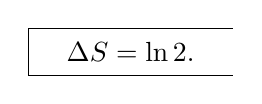
\begin{tikzpicture}
\node at (0,0) {$\Delta S=\ln2.$};
\draw (1.3,0.3)--(-1.3,0.3)--(-1.3,-0.3)--(1.3,-0.3);
\end{tikzpicture}
\end{adjustbox}
\end{center}

Следствие: потеря инф. $\Rightarrow$ рост энтропии

% Review acquisition-consequence: original pixels (260,1930)-(1170,2065).
Приобрет. инф. $\Rightarrow$ \Unclear{GELFAND-P000714}{acquisition-consequence}{уменьш. инф.}

Демон Максв. пониж. энтропию (следит за частицами)

Есть ли ещё способы потери инф.?

% Review forces-cancellation: original pixels (852,2244)-(1024,2311).
% Review before-volume-cancellation: original pixels (1800,2205)-(1873,2296).
Может быть, есть [зачёркнуто: \Unclear{GELFAND-P000714}{forces-cancellation}{неразборчиво}] силы, удерж. информацию [зачёркнуто: \Unclear{GELFAND-P000714}{before-volume-cancellation}{неразборчиво}] в д. объёме.

\underline{Изв. ситуация, когда информ. отсекается физич. средствами}

— не выходит инф.

Есть такая сила: \underline{тяготение}! (и она единственная)

Дальнодейств. и одного знака (!)

«Чёрная дыра» — тело, не выпускающ. информацию.

Придумал Лаплас: \underline{Скор. света $=2^{\underline{\text{й}}}$ космич. скор.}
\begin{equation*}
\frac{mv^2}{2}-\gamma\frac{mM}{R}=0
\end{equation*}
\begin{equation*}
\frac{mc^2}{2}=\gamma\frac{mM}{R},
\end{equation*}
\begin{equation*}
\fbox{$R=\dfrac{2\gamma M}{c^2}=r_g$}
\end{equation*}

При таком радиусе свет не покинет тело (и никакой сигнал)

— оказывается, верно и в точной теории
\SourcePage{GELFAND-P000715}{unlabelled}
\begin{equation*}
R_{\text{солнца}}=10^6\ \text{км}
\end{equation*}
[Зачёркнут знак: \Unclear{GELFAND-P000715}{mass-cancellation}{плотно зачёркнутый начальный знак; чтение не установлено.}]
Для его массы нужен рад. \underline{\underline{$7$ км.}}

О чёрной дыре принцип. ничего не можем знать, кроме неск. пар. —
— массы, заряда,
[зачёркнуто: \Incomplete{GELFAND-P000715}{charge-cancellation}{Слово между «заряда» и «радиуса» полностью перекрыто штрихами зачёркивания.}]
радиуса.

Как в случае газа. Микросост. огромное количество.
На самом деле это \underline{термодин. объект}!!

\underline{Хокинг}: [ниже имени: (раньше)] пов. чёрной дыры $S$ (!) возрастает при всех процессах.
Слияние 2-х чёрных дыр. Геом. ясно увелич. (из ф-мы Лапласа)

Буква $S$ сыграла замеч. роль.
\begin{equation*}
\underline{\frac{1}{T}=\frac{\partial S}{\partial E}}
\quad\Rightarrow\quad T\text{ — «темпер.» чёрной дыры.}
\end{equation*}
[Под левой формулой проведена скобка.]

\underline{Bekenstein} [под именем: (уч. Хокинга)] — снял кавычки!
Посчитал информацию, теряющуюся при постр. чёрных дыр!!
Совп. с энтр. информационной.

Кинем горячее тело на чёрную дыру. Оно увелич. пов.
больше, чем холодное, в точн. соотв. возраст. энтропии.

[Зачёркнуто: Хокинг.] \underline{\underline{Хокинг}}.
Слияние пар частиц. Чёрная дыра излучает и спектр планковский!
\begin{equation*}
\frac{1}{e^{\frac{\hbar\omega}{kT}}-1}
\end{equation*}
$T$ — та температура.

Информ. тер. не стохастизацией!!, а уходит в чёрные дыры.
(механич. отсекается)

Другие способы

\Unclear{GELFAND-P000715}{unruh-name}{Подчёркнутая латинская фамилия: Unruh / Uhru; точное начертание букв не установлено.}
Однор. поле тяготения.

Пусть в вакууме част. двиг. равномерно ускоренно.
До неё дойдёт свет не отовсюду.

\SourceFigure{GELFAND-P000715}{unruh-diagram}{Слева рисунок с вертикальной осью $t$ со стрелкой вверх и горизонтальной осью $x$ со стрелкой вправо; две диагонали пересекаются около начала координат. Справа от начала проведены наложенные кривые; имеются штриховка и стрелки. Точное соединение линий и принадлежность нескольких стрелок неразличимы.}

Получ., что свет дох. лишь от \underline{половины пр-ва}.
Наблюд. увидит (расчёт) \underline{планковское распред.}
Нулевые колеб. он видит перекошенными.
Это тяжёлый счёт.

$H$ — гам. эл.-магн. поля.
\begin{equation*}
H\,|\Phi\rangle=E_0\,|\varphi\rangle
\end{equation*}
\Unclear{GELFAND-P000715}{hamiltonian-state}{Слева знак состояния обведён и выглядит как $\Phi$, справа — как $\varphi$; различие начертаний сохранено, регистр не установлен окончательно.}

Вектор сост. с точки зр. неинерц. наблюд.
[Стрелка вправо к следующей записи.]
Счит. вер. $1^{\text{го}}$, $2^{\text{х}}$ и более

[Крайнее правое поле за вертикальной границей кадра:]
\Unclear{GELFAND-P000715}{outer-right-fragments}{Две группы обрезанных штрихов у самого правого края; отдельные знаки не читаются уверенно.}

\SourcePage{GELFAND-P000716}{42}
фотонов.
\begin{equation*}
\underline{kT=\frac{ha}{c}}\quad\Rightarrow\quad\text{температура}
\end{equation*}
[Под формулой проведена скобка.]
\Unclear{GELFAND-P000716}{temperature-constant}{Первый знак числителя выглядит как $h$; возможное чтение $\hbar$ не исключено. Формула и её коэффициент не исправлены.}

Нагрев. газа на финише.

\underline{Почему вселенная чёрная?}

[Слева:]
Эксперимент — остывает сейчас.
[Справа от этой заметки две вертикальные черты.]

[Справа:]
\underline{\underline{$T=3^{\circ}\mathrm{K}$}} — из распр.
[зачёркнуто: \Incomplete{GELFAND-P000716}{temperature-cancellation}{Слово перед «Планка» перекрыто несколькими штрихами зачёркивания.}]
Планка
излуч. из космоса.
[Под формулой: (реликтовое излучение)]

Область неизвестности была.
Возникла в какой-то момент времени. До этого бессмысленно
[ниже последнего слова: спрашивать].

\underline{Есть горизонт событий}.

\SourceFigure{GELFAND-P000716}{horizon-drawing}{Округлая замкнутая область с короткими лучеобразными штрихами снаружи; внутри точка, линии со стрелкообразными окончаниями и малые знаки. Начертание внутренних знаков и точные направления стрелок требуют сверки с источником.}
\underline{закрытая обл.} (свет не успел дойти оттуда).
($\Rightarrow$ поэтому для нас такая темпер.)

[Разделительная черта с точкой.]

Спонтанное наруш. симм.

\SourceFigure{GELFAND-P000716}{symmetry-curves}{Три наложенные кривые без осей и подписей: одна чашеобразная, две с боковыми впадинами. В центральной области линии перекрываются; точное продолжение каждой кривой через наложение не установлено.}

\underline{эволюция мин при}
\Unclear{GELFAND-P000716}{minimum-temperature}{Сокращение: «паден.» / «наруш.»; окончательное чтение не установлено.}
\underline{температуры}

[Разделительная черта с точкой.]

Идея \underline{Сени Вишика}, о том, почему сем. Гельфанда нестерилизован:
«Чтобы успешно проинтегрировать большую область, надо пользоваться
методом Монте-Карло».

\SourcePage{GELFAND-P000717}{55}
\underline{3/X-77 г.}\qquad \underline{Сем. Гельфанда.}

\begin{flushright}
Будет систематически: «некоммутативная\newline
алгебраическая геометрия»
\end{flushright}

\underline{Л. А. Дикий.}\qquad \underline{О новых алгебрах Ли.}

(\underline{Гельф., Дикий}, Функ. анализ, 11:2).

\underline{Def. 1.}\quad \underline{Алгебра $A$.}

[Справа зачёркнуто: В \Incomplete{GELFAND-P000717}{cancelled-top}{Дальнейшие буквы зачёркнутой записи неразборчивы.}]

\begin{equation*}
u_k^{(i)},\qquad k=0,1,\ldots,n;\qquad i=0,1,2,\ldots
\end{equation*}
\begin{equation*}
A=\left\{\sum a\,u_{k_1}^{(i_1)}u_{k_2}^{(i_2)}u_{k_3}^{(i_3)}\cdots u_{k_N}^{(i_N)}\right\},
\qquad a\in K\quad\text{(поле)},
\end{equation*}
\begin{flushright}
$A$ — алг. многочленов\newline
от образующих $u_k^{(i)}$\newline
\fbox{$A=K[u_k^{(i)}]$.}
\end{flushright}
\begin{equation*}
\xi=\sum a_{k,i}\frac{\partial}{\partial u_k^{(i)}},\qquad a_{k,i}\in A.
\end{equation*}
(сумма бесконечна).\qquad $\xi$ наз. дифференцированием
\begin{equation*}
\frac{d}{dx}=\sum_{k,i}u_k^{(i+1)}\frac{\partial}{\partial u_k^{(i)}}
\end{equation*}
\begin{equation*}
\frac{d}{dx}u_k^{(i)}=u_k^{(i+1)};\qquad
u_k^{(i)}=\left(\frac{d}{dx}\right)^i u_k;\qquad
u_k\underset{\mathrm{def}}{=}u_k^{(0)}
\end{equation*}

\underline{Def. 2.}\quad \underline{Пространство $\widetilde A$}\quad (пр-во функционалов)

В дальнейшем всегда $u_n=1$, $u_{n-1}=0$.
\begin{equation*}
\left\{f:\ \exists g,\ f=\frac{d}{dx}g\right\}=\frac{d}{dx}A;
\end{equation*}
\begin{equation*}
\widetilde A=A\big/\frac{d}{dx}A
\end{equation*}
\begin{equation*}
f\longmapsto f\bmod\frac{d}{dx}A=\widetilde f\in\widetilde A
\end{equation*}
\begin{equation*}
A\underset{\int\cdots\,dx}{\longrightarrow}\widetilde A
\qquad\qquad
\widetilde f=\int f\,dx
\end{equation*}

\underline{Задача.}
\begin{equation*}
f[u]\in\mathbb C[u_k^{(i)}];
\end{equation*}
\begin{equation*}
\int_{-\infty}^{\infty}f[u(x)]\,dx=0,\quad\forall u\in S(\mathbb R^1)
\quad\Longleftrightarrow\quad
f\in\frac{d}{dx}\mathbb C[u].
\end{equation*}

\underline{Def. 3.}\quad
$A^{n-1}={}$ пр-во наборов $(f_0,f_1,\ldots,f_{n-2})$, $f_k\in A$

[На левом поле: $\frac{\delta}{\delta u}$.]
\begin{equation*}
\frac{\delta}{\delta u}:\widetilde A\longrightarrow A^{n-1}
\end{equation*}
\begin{equation*}
\left(\frac{\delta\widetilde f}{\delta u}\right)_k
=\sum_{\ell=0}^{\infty}\left(-\frac{d}{dx}\right)^\ell
\frac{\partial f}{\partial u_k^{(\ell)}}
=\frac{\delta\widetilde f}{\delta u_k}.
\end{equation*}
(здесь $\widetilde f=f\bmod\frac{d}{dx}A$)

\SourcePage{GELFAND-P000718}{unlabelled}
\underline{Def. 4.}\quad $\ell:A^{n-1}\longrightarrow A^{n-1}$
\begin{equation*}
f=(f_0,\ldots,f_{n-2})
\end{equation*}
\begin{equation*}
(\ell f)_r=\sum_s\ell_{rs}f_s
\end{equation*}
\begin{equation*}
\begin{aligned}
\ell_{rs}&=\sum_{\gamma=0}^{n-1-r-s}
\Bigl[\binom{\gamma+r}{r}u_{r+s+\gamma+1}
\left(-i\frac{d}{dx}\right)^\gamma-\\
&\qquad-\binom{\gamma+s}{s}\left(i\frac{d}{dx}\right)^\gamma
u_{r+s+\gamma+1}\Bigr]
\end{aligned}
\end{equation*}
\Unclear{GELFAND-P000718}{operator-line-break}{[В конце первой строки и в начале второй стоят знаки минус.]}

\underline{$n=2,3$} просто;\qquad \underline{$n=4$} — 1-й содерж. пример.

\underline{Def. 5.}\quad $\forall f\in A^{n-1}$ построим
\begin{equation*}
\partial_f=\sum_{k,\ell}f_k^{(\ell)}\frac{\partial}{\partial u_k^{(\ell)}}
\qquad\text{(дифференцирование)}
\end{equation*}
Легко проверить, что
\begin{equation*}
\partial_f\frac{d}{dx}=\frac{d}{dx}\partial_f
\end{equation*}
Поэтому определена операция $\partial_f:\widetilde A\longrightarrow\widetilde A$.

\underline{Def. 6.}\quad Пусть $f,g\in A^{n-1}$. Положим
\begin{equation*}
([f,g])_r=\partial_f g_r-\partial_g f_r
\end{equation*}
Легко проверить, что
\begin{equation*}
[\partial_f,\partial_g]=\partial_{[f,g]}.
\end{equation*}
Поэтому коммутатор $[\cdot,\cdot]$ определяет на $A^{n-1}$ структуру
алгебры Ли.

\underline{Def. 7.}\quad опр. коммутатор в $\widetilde A$.
\begin{equation*}
\{\widetilde f,\widetilde g\}
=\int\sum_{r,s}\frac{\delta\widetilde f}{\delta u_r}\cdot
\ell_{rs}\frac{\delta\widetilde g}{\delta u_s}\,dx
\end{equation*}

\underline{Теорема:}
[Зачёркнуто: \Incomplete{GELFAND-P000718}{theorem-cancellation}{Слово под густой штриховкой неразборчиво.}]
\Unclear{GELFAND-P000718}{theorem-verb}{получается / получится} алгебра Ли

(т. е. выполнено тождество Якоби)

\underline{Задача:} доказать ее попроще.

\underline{С. П. Новиков}\qquad
$A=\frac{d^3}{dx^3}+\left(u\frac{d}{dx}+\frac{d}{dx}u\right)$

тоже задает алгебру Ли.

(и с помощью него можно записать ур-е КдФ).

\SourcePage{GELFAND-P000719}{56}
\underline{С. И. Гельфанд.} о раб. И. М. Гельф., И. Н. Бернш. и
\Unclear{GELFAND-P000719}{heading-final-word}{свои.}:

[Справа в рамке:]
«Локальная структура категории модулей Хариш-Чандры»
или «Некоммутативная алгебраическая геометрия I».

$G$ — вещественная группа Ли, полупростая

$K\subset G$, $K$ — максимальная компактная подгруппа

$\mathfrak g$ — алгебра Ли группы $G$

\underline{Определение.} Модуль Хариш-Чандры $M$ —
это линейное пр-во над $\mathbb C$ с действием $\mathfrak g$ и $K$ и с условиями
(кроме естеств. условий действия и согласования действий $\mathfrak g$ и $K$).

1) действия [зачёркнуто: алгебры Ли группы $K$] $\mathfrak g$ и $K$ согласованы:

а) алг. Ли $K$ действует на $M$ как подалгебра в $\mathfrak g$.

б) [зачёркнуто: \Unclear{GELFAND-P000719}{canceled-condition-label}{а)}]
\begin{equation*}
T\bigl(\underset{\substack{\uparrow\\K}}{k}\,
\underset{\substack{\uparrow\\\mathfrak g}}{X}\,k^{-1}\bigr)
=T_1(k)T(X)T_1(k^{-1}).
\end{equation*}
$T$ — действие $\mathfrak g$, $T_1$ — действие $K$

2) $M$ разбив. отн. $K$ в прямую сумму [вставлено над строкой: неприв.] представлений и
каждое [вставлено снизу: неприв.] предст. встречается конечное число раз.

М. Х.-Ч. обр. \underline{категорию}. Морфизмы определяются естеств. образом.

\underline{Задача:} описание этой категории.

\underline{Идея:} есть некоммут. алгебра, к-рая за это ответственна.

\underline{Гельфанд, Пономарев:} для группы Лоренца [вставлено снизу: $SL(2,\mathbb C)$]
свод. к классификации таких пар матриц $A,B$, что $AB=BA=0$,
[зачёркнуто: и
\Incomplete{GELFAND-P000719}{canceled-matrices}{Два последующих зачёркнутых слова не прочитаны.}]

$U(\mathfrak g)$ — обёртыв. алгебра $\mathfrak g$

$Z(\mathfrak g)$ — её центр

\begin{equation*}
M\rightsquigarrow J_M=\{z\in Z(\mathfrak g)\mid zM=0\}
\qquad\text{(идеал) в }Z(\mathfrak g).
\end{equation*}

$\Theta$ — множество характеров $\theta:Z(\mathfrak g)\to\mathbb C$.
(гомоморфизмов)

[Зачёркнуто под формулой: (линейные
\Unclear{GELFAND-P000719}{canceled-theta-abbrev}{ф-мы})]
$(\subset\mathbb C^N)$.
\Unclear{GELFAND-P000719}{theta-ambient-exponent}{Верхний индекс $N$ / $n$; в формуле показан первый кандидат, регистр не установлен.}

\begin{gather*}
\operatorname{supp}M\subset\Theta\\
\operatorname{supp}M=\{\theta\mid J_M\subset\ker\theta\}
\end{gather*}
$\operatorname{supp}M$ — конечное мн-во.

Пусть $D\subset\Theta$,
\begin{equation*}
C_D=\{M\mid\operatorname{supp}M\subset D\}.
\end{equation*}

\SourcePage{GELFAND-P000720}{unlabelled}
Можно рассм. модули Х.-Ч. с носит. в точке $C_{\{\theta\}}$

\underline{Теорема} (лёгкая).
[В следующей формуле после $C_D=$ зачёркнут одиночный знак:
\Unclear{GELFAND-P000720}{canceled-sum-symbol}{неразборчиво}.]
\begin{equation*}
C_D=\bigoplus_{\theta\in D}C_{\{\theta\}}
\end{equation*}
в нек-ром смысле,

(разлагаются и нет гомоморфизмов).

\underline{1-я основная теорема.} Пусть $D$ — огр. область в $\Theta$
(в компл. смысле). Тогда $\exists\ Z(\mathfrak g)$-алгебра $Q$
[справа внизу зачёркнуто: \Unclear{GELFAND-P000720}{algebra-canceled-sign}{неразборчивый знак}]
[зачёркнуто: такая]
с конечным числом $a$ аддитивных $Z(\mathfrak g)$-образующих,
[вставлено над строкой: такая что]
[зачёркнуто: \Unclear{GELFAND-P000720}{canceled-theorem-word}{Тогда}]
$C_D$ эквивалентна категории $Q$-модулей, которые конечномерны над $\mathbb C$.

($\exists$ функтор, осущ. эквивалентность)

$Q$ — $Z(\mathfrak g)$

\begin{center}— · —\end{center}

«Известия» [под названием: 23/$\overline{\underline{\mathrm{IX}}}$-77]
и «Соц. индустрия» [под названием: 22/$\overline{\underline{\mathrm{IX}}}$-77]
[зачёркнуто: от 23]

сообщение из Петрозаводска о неопознанном летающем объекте

\begin{center}— · —\end{center}

\underline{Пример.}
\begin{gather*}
G=SL_2(\mathbb R)/\{\pm1\}\\
Z(\mathfrak g)\cong\mathbb C[z]\\
\Theta=\mathbb C^1
\end{gather*}

\begin{center}
\begin{adjustbox}{max width=\linewidth}
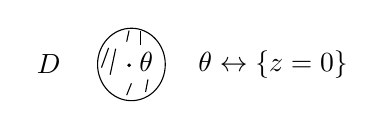
\begin{tikzpicture}
\node at (-1.05,0) {$D$};
\draw (0,0) ellipse (0.43 and 0.46);
\draw (-0.27,-0.13) -- (-0.20,0.20);
\draw (-0.38,-0.04) -- (-0.29,0.21);
\draw (-0.06,0.29) -- (-0.03,0.43);
\draw (0.12,0.25) -- (0.12,0.43);
\draw (-0.06,-0.39) -- (0.00,-0.24);
\draw (0.18,-0.35) -- (0.21,-0.19);
\fill (-0.03,-0.01) circle (0.025);
\node at (0.19,0.03) {$\theta$};
\node at (1.80,0) {$\theta\leftrightarrow\{z=0\}$};
\end{tikzpicture}
\end{adjustbox}
\end{center}

Алгебру будем строить над аналит. ф-ями
\begin{equation*}
Q=(a_{ij}(z))_{i,j=1}^{3}\text{ — матр. }3\times3,
\qquad a_{ij}(z)\text{ — целые ф-и}
\end{equation*}
\begin{equation*}
(a_{ij}(0))=
\begin{pmatrix}
*&0&0\\
*&*&0\\
*&0&*
\end{pmatrix}
\end{equation*}

\SourcePage{GELFAND-P000721}{unlabelled}
\underline{10/$\overline{\underline{\mathrm X}}$-77 г.}
\qquad\underline{\underline{Сем. Гельфанда.}}

\underline{С. Гельфанд.}

$G$ — полупростая вещественная группа Ли

$K$ — максимальная компактная подгруппа

$\mathfrak g$ — алгебра Ли группы $G$

$U(\mathfrak g)$ — обёртывающая алгебра.

$Z(\mathfrak g)$ — центр $U(\mathfrak g)$

Модуль Хариш-Чандры (МХЧ) $V$, если

[\underline{Теор. Х.-Ч.:} в непривод. предст. полупростой группы каждое
[вставлено сверху: неприв.] предст. макс. комп. группы $K$ встреч. конечн. число раз]

В $V$ заданы предст. $T_1$ алг. $U(\mathfrak g)$, $T_2$ — предст. группы $K$.

1) $V$ — конечно порожд. $U(\mathfrak g)$-модуль.

2) $\left.T_1\right|_{\mathfrak k}=dT_2$,
\begin{equation*}
T_2(k)T_1(X)T_2(k^{-1})=T_1(kXk^{-1})
\end{equation*}

3) $T_2=\bigoplus$ неприв. непр. предст. $K$, причём каждое встречается конечное число раз.

(прямая сумма в букв. смысле).

[Зачёркнуто:
\Incomplete{GELFAND-P000721}{canceled-result-heading}{Плотно зачёркнутая запись перед словом «Результат» не прочитана.}]

\underline{Результат:} пусть
\begin{equation*}
\Theta=\{\theta:Z(\mathfrak g)\to\mathbb C\}=\mathbb C^{r}
\end{equation*}
\Unclear{GELFAND-P000721}{theta-exponent}{Верхний индекс $r$ / $\tau$; в формуле показан первый кандидат, чтение не установлено.}
(кольцевые гомоморфизмы)

\begin{equation*}
V\mapsto\operatorname{supp}V\subset\Theta
\end{equation*}

\begin{equation*}
\theta(z)\in\operatorname{supp}V
\Longleftrightarrow\exists\underset{\substack{\uparrow\\V}}{v}:
T_1(z)v=\theta(z)v,\quad z\in Z(\mathfrak g)
\end{equation*}
\Unclear{GELFAND-P000721}{support-criterion}{В источнике написано $\theta(z)\in\operatorname{supp}V$ и нет явного условия $v\ne0$; запись сохранена без исправления.}

На самом деле [зачёркнуто:
\Incomplete{GELFAND-P000721}{canceled-support-symbol}{Короткая запись под вставкой «supp V —» не прочитана.}]
[вставлено над строкой: $\operatorname{supp}V$ —] конечное мн-во.

Пусть есть огр. область $D\subset\Theta$,
\begin{equation*}
C_D=\{V:\operatorname{supp}V\subset D\}.
\end{equation*}
Для непересек. мн-в $D_1$ и $D_2$ получ. прямая сумма категорий.

\underline{Эквивалентность категорий:}
\begin{center}
\begin{adjustbox}{max width=\linewidth}
\begin{tikzcd}
\mathcal A\arrow[r,shift left,"\varphi"]&
\mathcal B\arrow[l,shift left,"\psi"]
\end{tikzcd}
\end{adjustbox}
\end{center}

$\varphi,\psi$ — функторы

\begin{equation*}
\varphi\circ\psi\underset{\uparrow}{\sim}\operatorname{id}_B,
\qquad
\psi\circ\varphi\underset{\nearrow}{\sim}\operatorname{id}_A
\end{equation*}
[К обоим знакам $\sim$ проведены стрелки от надписи:]
изоморфизм
[зачёркнуто:
\Incomplete{GELFAND-P000721}{bottom-cancellation}{Слово между «изоморфизм» и «функторов» не прочитано из-за плотного зачёркивания.}]
функторов

\SourcePage{GELFAND-P000722}{unlabelled}
\Incomplete{GELFAND-P000722}{whole-frame}{Исходный PNG не проходит проверку и декодирование: Truncated File Read. Надёжное изображение кадра недоступно; текст не восстанавливался.}

\SourcePage{GELFAND-P000723}{unlabelled}
\underline{Условие, выделяющее $R$:}
\begin{equation*}
a_{ij}(0)=
\begin{pmatrix}
\ast&0&0\\
\ast&\ast&0\\
\ast&0&\ast
\end{pmatrix}
\end{equation*}

\underline{Есть над ф-ями базис из 9 элементов.}
\begin{equation*}
e_{11}=
\begin{pmatrix}
1&0&0\\
0&0&0\\
0&0&0
\end{pmatrix},\quad
e_{12}
\begin{pmatrix}
0&z&0\\
0&0&0\\
0&0&0
\end{pmatrix},\quad
e_{21}=
\begin{pmatrix}
0&0&0\\
1&0&0\\
0&0&0
\end{pmatrix}
\end{equation*}
\Unclear{GELFAND-P000723}{basis-e12-leading-zero}{В начальном нуле матрицы $e_{12}$ видны внутренние штрихи; предшествующий начерк не установлен.}
и т. д.
\Unclear{GELFAND-P000723}{basis-e12-gap}{[Между $e_{12}$ и матрицей знак равенства не виден.]}

\begin{equation*}
\underline{e_{21}e_{12}=ze_{22}}
\end{equation*}

Хотим найти конечномерные модули, чтобы умн. на $z$
было нильпот. оператором.
\begin{equation*}
\underline{e_{ii}^{2}=e_{ii}}.
\end{equation*}
\begin{equation*}
L_i=\{m:\ e_{ii}m=m\}.
\end{equation*}
\begin{equation*}
M=L_1\oplus L_2\oplus L_3
\end{equation*}

\begin{center}
\begin{adjustbox}{max width=\linewidth}
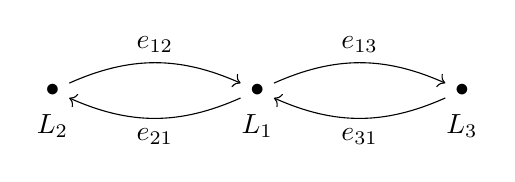
\begin{tikzpicture}
\node (l2) at (0,0) {$\bullet$};
\node (l1) at (2.6,0) {$\bullet$};
\node (l3) at (5.2,0) {$\bullet$};
\node at (0,-0.45) {$L_2$};
\node at (2.6,-0.45) {$L_1$};
\node at (5.2,-0.45) {$L_3$};
\draw[->] (l2) to[bend left=24] node[above] {$e_{12}$} (l1);
\draw[->] (l1) to[bend left=24] node[below] {$e_{21}$} (l2);
\draw[->] (l1) to[bend left=24] node[above] {$e_{13}$} (l3);
\draw[->] (l3) to[bend left=24] node[below] {$e_{31}$} (l1);
\end{tikzpicture}
\end{adjustbox}
\end{center}
\Unclear{GELFAND-P000723}{diagram-right-directions}{[Направления стрелок $e_{13}$ и $e_{31}$ сохранены по рукописи.]}

\begin{equation*}
e_{21}e_{12}=ze_{22}\qquad\text{нильпотентен}
\end{equation*}
\begin{equation*}
e_{12}e_{21}=ze_{11}=e_{13}e_{31}
\end{equation*}
отсюда катег. модулей над этим кольцом $\cong\ldots$

\underline{\underline{Для $SL(3,\mathbb R)$}}\qquad
\underline{ответ таков:}
\begin{equation*}
E=\{z_1,z_2\}\qquad\text{в окр. нуля:}
\end{equation*}
\begin{equation*}
B=\underset{a_{ij}}{M_4}\oplus
\underset{b_{ij}}{M_3}\oplus
\underset{c_{ij}}{M_3}\oplus
\underset{d}{M_1}
\end{equation*}
\underline{Условия.}
\begin{equation*}
1)\ \text{При }z_1=0\qquad\left\Vert\quad
\begin{aligned}
a_{13}=a_{14}=a_{23}=a_{24}=b_{12}=b_{13}=0\\
a_{33}=b_{22},\quad a_{34}=b_{23},\quad
a_{43}=b_{32},\quad a_{44}=b_{33}
\end{aligned}\right.
\end{equation*}

\SourcePage{GELFAND-P000724}{62}
\begin{center}
\begin{adjustbox}{max width=\linewidth}
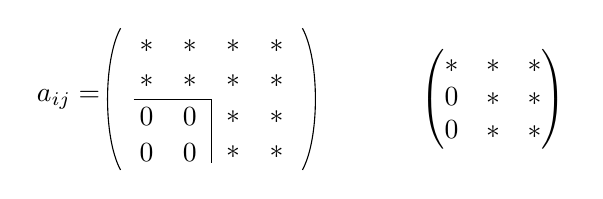
\begin{tikzpicture}[x=0.55cm,y=0.45cm]
\node at (-1.8,-1.5) {$a_{ij}=$};
\node at (0,0) {$\ast$};
\node at (1,0) {$\ast$};
\node at (2,0) {$\ast$};
\node at (3,0) {$\ast$};
\node at (0,-1) {$\ast$};
\node at (1,-1) {$\ast$};
\node at (2,-1) {$\ast$};
\node at (3,-1) {$\ast$};
\node at (0,-2) {$0$};
\node at (1,-2) {$0$};
\node at (2,-2) {$\ast$};
\node at (3,-2) {$\ast$};
\node at (0,-3) {$0$};
\node at (1,-3) {$0$};
\node at (2,-3) {$\ast$};
\node at (3,-3) {$\ast$};
\draw (-0.6,0.5) .. controls (-1,-0.4) and (-1,-2.6) .. (-0.6,-3.5);
\draw (3.6,0.5) .. controls (4,-0.4) and (4,-2.6) .. (3.6,-3.5);
\draw (-0.3,-1.5) -- (1.5,-1.5) -- (1.5,-3.3);
\node at (8,-1.5) {$\begin{pmatrix}\ast&\ast&\ast\\0&\ast&\ast\\0&\ast&\ast\end{pmatrix}$};
\end{tikzpicture}
\end{adjustbox}
\end{center}
\Unclear{GELFAND-P000724}{top-matrix-consistency}{[Расположение нулей в матрицах сохранено по рукописи.]}

\begin{equation*}
2)\ \text{При }z_2=0\qquad\left\Vert\quad
\begin{aligned}
a_{12}=a_{14}=a_{34}=c_{12}=c_{13}=a_{32}=0\\
a_{22}=c_{22},\quad a_{24}=c_{23},\quad
a_{42}=c_{32},\quad a_{44}=c_{33}
\end{aligned}\right.
\end{equation*}

3) При $z_1$ \Unclear{GELFAND-P000724}{condition-three-sign}{$+$ / $\ne$; окончательный знак не установлен.} $z_2=0$.
\begin{equation*}
\left\Vert\quad
\begin{aligned}
b_{13}=b_{23}=c_{13}=c_{23}=0;\\
b_{33}=c_{33}.
\end{aligned}\right.
\end{equation*}
\SourcePage{GELFAND-P000725}{unlabelled}
\underline{24/Х--77 г.}

\underline{С. И. Гельфанд.}\qquad
\underline{Модули Хариш--Чандры}

МХЧ для
\begin{equation*}
G=SL(2,\mathbb{R})/(\pm1),\qquad
K=SO_2/(\pm1)
\end{equation*}
(макс. комп. подгруппа)

$\mathfrak{g}$ --- алгебра Ли
\begin{equation*}
\begin{array}{ccc}
E_+,&E_-,&H\\
\begin{pmatrix}0&1\\0&0\end{pmatrix},&
\begin{pmatrix}0&0\\1&0\end{pmatrix},&
\begin{pmatrix}1&0\\0&-1\end{pmatrix}
\end{array}
\qquad\text{--- образующие }\mathfrak{g}.
\end{equation*}
\begin{equation*}
\begin{array}{cl}
\mathfrak{k}&\subset\mathfrak{g}.\\
\Vert&\\
\left\{\begin{pmatrix}0&1\\-1&0\end{pmatrix}=
X_c\right\}&
\end{array}
\end{equation*}
\Unclear{GELFAND-P000725}{bottom-generator}{$X_c$; $X_0$?}
\SourcePage{GELFAND-P000726}{67}
\underline{Модуль} Х.--Ч. --- такое (бесконечномерное) предст. в
[зачеркнуто: \Unclear{GELFAND-P000726}{top-cancellation}{неразборчиво}]
$V$, что

1) $X_0$ имеет лишь целочисленные соб. значения и притом чётные.

2) [зачеркнуто: \Unclear{GELFAND-P000726}{item-two-cancellation}{неразборчиво}]
каждое собств. значение [вставлено: оператора $X_0$] конечнократно

3) $V$ конечно порождён (над обёрт. алгеброй)

($\Leftrightarrow$ кратности соб. значений ограничены).

$v_1,\ldots,v_n$ --- образующие

[На правом поле, отделено двойной чертой:]
1) --- чтобы можно было проинтегрировать до предст. группы
($e^{inx}$ и т. д.)

\underline{Определение.}\quad $Z(\mathfrak{g})$ --- центр обёрт. алгебры $U(\mathfrak{g})$

(порожд. элементом
\Unclear{GELFAND-P000726}{casimir-sign}{$z=4E_-E_+-H^2+2H$})

$\operatorname{supp}V={}$ мн-во собств. значений оператора $z$ в $V$

\underline{Теорема:} это конечное мн-во для любого $V$.

\underline{Определение.} Пусть $D$ --- область в $\mathbb{C}$.
\begin{equation*}
C_D=\{V,\ \operatorname{supp}V\subset D\}
\end{equation*}
Пусть $D$ --- маленькая окрестность нуля (круг радиуса $<1/2$).
\begin{equation*}
R=\left\{
\begin{pmatrix}
a_{11}(\lambda)&a_{12}(\lambda)&a_{13}(\lambda)\\
a_{21}(\lambda)&a_{22}(\lambda)&a_{23}(\lambda)\\
a_{31}(\lambda)&a_{32}(\lambda)&a_{33}(\lambda)
\end{pmatrix}\right.,\quad
 a_{ij}(\lambda)\text{ --- аналит. ф-и в }D
\end{equation*}
\begin{equation*}
a_{ij}(0)=
\begin{pmatrix}*&0&0\\ *&*&0\\ *&0&*\end{pmatrix}
\end{equation*}
\Unclear{GELFAND-P000726}{matrix-value-notation}{Слева записано $a_{ij}(0)$ без скобок вокруг набора элементов.}
\begin{equation*}
\operatorname{Mod}R=\{\underset{\substack{\uparrow\\R\text{-модуль}}}{M}:\ \dim_{\mathbb{C}}M<\infty\}
\end{equation*}
\underline{Теорема.} Категория $C_D$ эквивалентна категории $\operatorname{Mod}R$.

\underline{Пример.}

\underline{Категория модулей над кольцом матриц эквивалентна}
\underline{категории} [зачеркнуто:
\Unclear{GELFAND-P000726}{cancelled-category}{линейных?}]
\underline{конечномерных линейных пространств}

($\sim$ предст. алг. матриц --- прямая сумма)

$V$ --- станд. предст. алг.
\Unclear{GELFAND-P000726}{matrix-subscript}{$M_\ell$; $M_e$?}
\begin{equation*}
E\longmapsto V\underset{\mathbb{C}}{\otimes}E,\qquad
M_\ell\text{ действ. по 1-му переменному}
\end{equation*}
\begin{equation*}
W\text{ --- }M_\ell\text{-модуль}\quad\longmapsto\quad
E=\operatorname{Hom}_{M_\ell}(V,W).
\end{equation*}
(выписаны 2 функтора, задающие эквивалентность)

Старая формулировка: $\forall\ M_\ell$ модуль разлагается в прямую сумму.
\SourcePage{GELFAND-P000727}{unlabelled}
\underline{Док-во теоремы.}

I. Пусть дан набор чисел $n_1,\ldots,n_k$. Построим по нему
кольцо $Q_{n_1,\ldots,n_k}$

а) $J_{n_1\ldots n_k}$ --- левый идеал в $U(\mathfrak{g})$, порождённый элементом
\begin{equation*}
(X_0-2in_1)(X_0-2in_2)\cdots(X_0-2in_k)
\end{equation*}

б)
\begin{equation*}
N_{n_1,\ldots,n_k}=\{u\in U(\mathfrak{g})\mid
J_{n_1,\ldots,n_k}u\subset J_{n_1,\ldots,n_k}\}
\end{equation*}
(\Unclear{GELFAND-P000727}{normalizer-word}{наименьшая подалг.}, в к-рой $J$ --- 2-стор. идеал
\begin{equation*}
Q_{n_1\ldots n_k}=N_{n_1,\ldots,n_k}/J_{n_1,\ldots,n_k}
\end{equation*}

\underline{Опрд.}\quad $V$ --- модуль Х.--Ч.
\begin{equation*}
\tau_{n_1,\ldots,n_k}(V)\underset{\mathrm{def}}{=}
\{v:\ (X_0-2in_1)\cdots(X_0-2in_k)v=0\}
\end{equation*}
Это конечномерное подпр-во

Размерность $={}$ сумме кратностей

$N$ переводит его в себя

$J$ \quad --- '' --- \quad в нуль
\begin{equation*}
\Rightarrow\quad Q_{n_1,\ldots,n_k}\text{ действует в }\tau_{n_1,\ldots,n_k}(V)
\end{equation*}
Это [зачеркнуто:
\Unclear{GELFAND-P000727}{functor-cancellation}{категория?; конструкция?}]
функтор
\begin{equation*}
\text{Модули Х.--Ч.}\longrightarrow
\text{конечномерные модули над }Q_{n_1,\ldots,n_k}
\end{equation*}
Ясно, что
\begin{equation*}
z\in N_{n_1,\ldots,n_k}
\end{equation*}
\begin{equation*}
\operatorname{supp}M=\{\text{соб. значения }z\}
\end{equation*}
\begin{equation*}
(\operatorname{Mod}Q_{n_1,\ldots,n_k})_D
\end{equation*}
(конечномерные модули с носителем в $D$)

\SourceFigure{GELFAND-P000727}{bottom-arrow}{Между пояснением о носителе и строкой теоремы, над словом «область», небольшой знак: стрелка влево, справа поперечная черта; привязка к тексту неясна.}

\underline{Теорема 1.} Пусть $D$ --- любая огр. область в $\mathbb{C}^1$. Тогда
сущ. $n_1,\ldots,n_k$, такие что $C_D$ и
$(\operatorname{Mod}Q_{n_1,\ldots,n_k})_D$ эквив.
\SourcePage{GELFAND-P000728}{68}
\underline{II. Определение предст. основной серии.}

по $s$ постр. модуль $T^{(s)}=V$
\begin{equation*}
V=\{\underset{\substack{\text{функции}\\\text{на плоск.}}}{f(x,y)}\}
\end{equation*}
1) $f(tx,ty)=|t|^sf(x,y)$

2) $f(+\sin\varphi,\cos\varphi)=P(\sin\varphi,\cos\varphi)$

$\underline{P}$ --- многочлен.

Алгебра Ли действ. естеств. образом (дифф. операторы)

(группа --- на аргумент)
\begin{equation*}
E_+\sim x\frac{\partial}{\partial y};\quad
E_-\sim y\frac{\partial}{\partial x};\quad
H\sim x\frac{\partial}{\partial x}-y\frac{\partial}{\partial y}.
\end{equation*}
Огранич. на $S^1\cong{}$ пр-во многочленов (чётных на окружности)
\begin{equation*}
L_0\simeq T^{(s)}\qquad\text{(при любом }s\text{).}
\end{equation*}
\underline{Лемма 1.} Пусть $X\in U(\mathfrak{g})$. Действие $X$ полиномиально
зависит от $s$.

(Матричные элементы в базисе одночленов --- полиномы от $s$)
\begin{equation*}
\tau_{n_1,\ldots,n_k}(T^{(s)})=L_{n_1,\ldots,n_k}
\end{equation*}
\underline{Лемма 2.} Пусть $q\in Q_{n_1,\ldots,n_k}$. Действие $q$ полиномиально
зависит от $s$.

\underline{Теорема 2.}\quad \underline{Положим}
\begin{equation*}
B_{n_1,\ldots,n_k}=\operatorname{End}(L_{n_1,\ldots,n_k})
\end{equation*}
Тогда существует отображение
\begin{equation*}
\psi_{n_1,\ldots,n_k}:
Q_{n_1,\ldots,n_k}\longrightarrow B_{n_1,\ldots,n_k}[s],
\end{equation*}
\Unclear{GELFAND-P000728}{embedding-symbol}{$\psi_{n_1,\ldots,n_k}$; $\Psi$?; $\gamma$?}
[зачеркнуто: \Unclear{GELFAND-P000728}{embedding-cancellation}{Теор.?; Тогда?};
сверху вставлено: так что]
$\psi$ --- \underline{вложение}

(т. е. в основной серии в кач. под- и фактор- предст. содерж.
$\forall$ МХЧ)

\underline{III. Объед. I и II этапов.}

$D$ --- маленькая окр. нуля

\underline{Лемма 0.}

На $T^{(s)}$ оператор $z$ есть
\Unclear{GELFAND-P000728}{scalar-casimir}{$(-s^2+2s)\operatorname{Id}$}

$z=0$ при $s=0$ и $s=2$.

\underline{Лемма 1.} Пусть $s$ вблизи точки 0.

1) Тогда $T^s$, $s\ne0$ неприводимо
\begin{equation*}
0\longrightarrow\operatorname{Id}\longrightarrow T^{(0)}
\longrightarrow T_+\oplus T_-\longrightarrow0
\end{equation*}
и точн. послед. не расщепляется
\SourcePage{GELFAND-P000729}{unlabelled}
2)
\begin{equation*}
T^{(s)}\big|_K=\bigoplus_{j=-\infty}^{\infty}\delta_j
\end{equation*}
$\delta_k$ --- соб. подпр. $X_0$ с соб. знач. $2ik$.

(1-мерное предст.)
\begin{equation*}
I\big|_K=\delta_0,\qquad
T_+\big|_K=\bigoplus_{j>0}\delta_j,\qquad
T_-\big|_K=\bigoplus_{j<0}\delta_j
\end{equation*}
[На левом поле: В]

\underline{Лемма 2.} Вблизи $s=2$
\begin{equation*}
0\longrightarrow T_+\oplus T_-\longrightarrow T^{(2)}\longrightarrow I\longrightarrow0
\end{equation*}
$T^{(s)}$, $s\ne2$ неприводимо

\underline{Лемма 3.}\quad $s\ne0$\quad $T^{(s)}\simeq T^{(2-s)}$

$s$ вблизи нуля

Рассмотрим числа $(n_1,n_2,n_3)=(-1,0,1)$ и кольцо
\begin{equation*}
Q_{(-1,0,1)}
\end{equation*}
$D$ --- дост. малая окр. нуля\quad $\Rightarrow\quad C_D\sim Q_{(-1,0,1)}$

(\underline{объяснение:} в $T_+$ есть предст. с $+1$, в $T_-$ --- '' --- с $-1$ и т. д.)
\begin{equation*}
\tau_{-1,0,1}(T^{(s)})=\{e_{-1},e_0,e_1\}
\end{equation*}
$q\in Q_{-1,0,1}$

[Точечная разделительная линия.]

\underline{Сделано:}\quad $SL(2,\mathbb{R})/(\pm1)$,\quad $SL(2,\mathbb{R})$,\quad $PGL(2,\mathbb{R})$,

$SL(2,\mathbb{C})$, $SL(3,\mathbb{R})$

Наверное, можно $SL(3,\mathbb{C})$ и $SU(2,1)$

Рекомендуется, сосчит. $SO(4,1)$ (легко), $Sp(4,\mathbb{C})$ (легко)

Трудно: $SL(4,\mathbb{R})/(\pm1)$, $SL(4,\mathbb{C})$.

Читать: раб. Хираи; Желобенко

Гельфанд, Граев

\underline{Кричевер}

\underline{2 минуты для сенсационного сообщения.}

[На левом поле: \underline{\Unclear{GELFAND-P000729}{margin-abbreviation}{Об ур-и; Об ур-й?}}]
\begin{equation*}
[L_1,L_2]=0
\end{equation*}
Коддингтон указал на раб.

\underline{Burchnal}, \underline{Chaundy}\quad 1922, 1928, 1931

и \underline{Baker} [зачеркнуто: \Unclear{GELFAND-P000729}{baker-cancellation}{неразборчиво}] 1928

[Справа от списка работ:] --- возразили Baker'у, к-рый рекомендовал польз. алг. геом.

Поставлена и решена задача об описании коммут. опр. со скал.
коэфф. взаимно простого пор.

ответ не через $\Theta$-ф-и и не достаточно эффективен

1-й через ф-и Ламе нашли (как Ахиезер). не увидели прямолин.
\SourcePage{GELFAND-P000730}{69}
пути на якобиане (и даже условной периодичности).

Забыли --- в раб. 1939 ссылок уже нет.

Proc. Lond. Math. Soc. 1922.

Proc. Royal Soc. --- остальные

[Слева возле двух строк Proc. --- вертикальные скобки с поперечными концами.]

почти коммутир. и пары Лакса \underline{есть}.

[Перед датой зачеркнуто:
\Unclear{GELFAND-P000730}{date-cancellation}{неразборчиво}]

\underline{31/Х--77 г.}\quad \underline{Сем. Гельфанда.}\quad
\underline{С. П. Новиков.}\quad \underline{Инстантоны.}
\begin{equation*}
\mathbb{R}^4\subset S^4\qquad(|x|\to\infty)
\end{equation*}
\begin{equation*}
A=A_\mu\,dx^\mu\qquad\text{форма связности}
\end{equation*}
[В формуле после знака равенства зачеркнуто:
\Unclear{GELFAND-P000730}{connection-cancellation}{$A_\mu\,d\mu$?; $A_\mu\,dx^\mu$?}]

Если кривизна равна 0, то
\begin{equation*}
A_\mu\longrightarrow\frac{\partial g}{\partial x^\mu}\,g^{-1}(x),\qquad
 g(x)\in G\tag{1}
\end{equation*}
\begin{equation*}
A_\mu(x)\in L_G\qquad\text{(алгебра Ли)}
\end{equation*}
Форма кривизны:
\begin{equation*}
F_{\nu\mu}=dA+[A,A]=\mathcal{D}A\tag{2}
\end{equation*}
(ковариантная производная)

Чаще всего $G=SU_2$ (Янг--Миллс).

$[A,A]$ --- внешнее произв., но умн. коэфф. --- в алг. Ли.

Другие обозначения: $A\wedge A=[A,A]$,\quad $\mathcal{D}A=\nabla_AA$

Требование, что всё на $S^4$ --- чуть сильнее конечности энергии.

(\underline{Замеч.}
Нелинейные (киральные) поля $\leftrightarrow$ связность с 0-й кривизной,
задаётся ф-ями со знач. в группе.)

Положим
\begin{equation*}
n=P(A)=\frac12\int\varepsilon_{abcd}F^{ab}F^{cd}\,d^4x\tag{3}
\end{equation*}
\Unclear{GELFAND-P000730}{topological-integral}{В (3) след или иная свёртка по матричным индексам явно не выписаны.}
(хар. класс Черна --- топ. инвариант --- целое число с точн. до
множителя \Unclear{GELFAND-P000730}{chern-factor}{$\pi^2/16$; $\pi^2/20$?}).
\begin{equation*}
S(A)=\frac{1}{g_0}
\int_{\mathbb{R}^4}\operatorname{Sp}(F_{\mu\nu}F^{\mu\nu})\,d^4x\tag{4}
\end{equation*}
\Unclear{GELFAND-P000730}{coupling-subscript}{В коэффициенте (4) $g_0$; $g_c$?}
(ф-л Янга--Миллса)

\underline{Классич. эл.-динамика} ---
\Unclear{GELFAND-P000730}{electrodynamics-group}{$G=SU(1)$} или $\mathbb{R}$

в завис. от того, есть \Unclear{GELFAND-P000730}{charges-adjective}{реал.; рац.?} заряды или нет.

Ур-я Янга--Миллса:
\begin{equation*}
\delta S=0.\tag{5}
\end{equation*}
Классич. задача: найти все такие $A$, что $S(A)<+\infty$.

\underline{Замеч.} Метрика $S^4$ конформно эквив. метрике $\mathbb{R}^4$,
\begin{equation*}
g_{\mu\nu}(y)=g(y)\delta_{\mu\nu}
\end{equation*}
Ур-я Максвелла и Янга--Миллса \underline{конформно инвариантны}.

Гр. конформных преобр. евкл. пр-ва и сферы\quad $\Vert\quad O(5,1)=K_4$
\SourcePage{GELFAND-P000731}{unlabelled}
Решения умн. на скаляр под действ. конформной группы:
\begin{equation*}
f:X\longrightarrow X,\qquad f^*(g_{ij})=g(x)g_{ij}.
\end{equation*}
(\Unclear{GELFAND-P000731}{parenthesis-word}{непрерывные?} конф. преобр.)

[Зачеркнуто: \Unclear{GELFAND-P000731}{top-cancellation}{Непр. рассл. в?}]

Непр. отобр. баз переводит рассл. в рассл. и связность в связность.
Тогда новая связность снова удовл. ур-ю Янга--Миллса.

$\underline{O(5,1)}$

На сфере $S^4$ есть $O(5)$

Стереогр. преобр. $S^4$ на $\mathbb{R}^4$ и в $\mathbb{R}^4$ берём подобные преобр.

Откуда $O(5,1)$?

Надо рассм. конус
\begin{equation*}
\underline{x_1^2+x_2^2+\cdots+x_5^2-x_6^2=0.}
\end{equation*}
\begin{adjustbox}{max width=\linewidth}
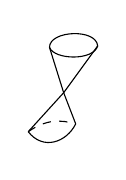
\begin{tikzpicture}[scale=0.9]
\draw (-0.20,0.64) .. controls (-0.20,0.88) and (0.46,0.91) .. (0.48,0.66)
 .. controls (0.42,0.45) and (-0.13,0.46) .. (-0.20,0.64);
\draw (-0.20,0.64) -- (0,0) -- (0.17,-0.44);
\draw (0.48,0.66) -- (0,0) -- (-0.50,-0.55);
\draw (-0.50,-0.55) .. controls (-0.29,-0.82) and (0.04,-0.70) .. (0.17,-0.44);
\draw[dashed] (-0.50,-0.55) .. controls (-0.24,-0.37) and (-0.04,-0.38) .. (0.17,-0.44);
\end{tikzpicture}
\end{adjustbox}

\Unclear{GELFAND-P000731}{cone-caption-symbol}{неразборчивый знак; $\mathbb{R}$?}
и лин. преобр., сохр. конус.

Лучи конуса --- $S^4$. Преобр. конформные на $S^4$.

Конформная группа сохр. ф-л $S(A)$

\underline{Инстантоны Белавина--Полякова.}
\begin{equation*}
\min_{P(A)=n}S(A)=n.\qquad
\text{(при }g_0=1\text{)}\tag{6}
\end{equation*}
\Unclear{GELFAND-P000731}{coupling-condition}{В условии при (6) $g_0=1$; $g_c$?}
и на самом деле минимумы удовл. ур-ю
[зачеркнуто: \Unclear{GELFAND-P000731}{equation-cancellation}{$F=*F$?}]
\begin{equation*}
\underline{F=*F}\tag{7}
\end{equation*}
(ур-я дуальности)

(Белавин и Поляков)

И обратное, реш. этих ур-й с данным $n$ --- реализ. строгий минимум в данном классе.

Явно представили ряд авторов (для $\forall\ n$ хотя бы одно решение).

[Зачеркнуто: \Unclear{GELFAND-P000731}{hooft-cancellation}{Гер?}]
\underline{t' Hooft} нашёл явные ф-лы при \underline{$n=2$}. (все решения!)

с пом. элем. подстановки.

Решения обр. $(8n-3)$-мерное многообразие (Шварц из теор. Атьи--Зингера).
Это $M^{8n-3}$.

Атья--Зингер на 3 месяца позже.

t' Hooft нашёл [зачеркнуто: \Unclear{GELFAND-P000731}{family-cancellation}{се?}]
м-ие размерности $\underline{5n+4}$. ($n\ge3$)

При $n=2$ совпадают. Не ясно, нет ли ещё связной компоненты.

\underline{Д-во теор. Шварца}

Линеаризуем ур-я (7):
\begin{equation*}
(A_\mu)\longrightarrow A_\mu+a_\mu=A+\delta A
\end{equation*}
линеариз. оператор\quad $a_\mu\longrightarrow Ta_\mu$
\SourcePage{GELFAND-P000732}{70}
\begin{equation*}
B(A)=F-*F=0,\qquad
B(A+\delta A)=T(\delta A)+O((\delta A)^2).
\end{equation*}
\underline{Счёт индекса}: $cn$ — линейная ф-я от $n$; считается знач. в $0$ и $1$.

\underline{\underline{Коядро $=0$}}
[Зачёркнуто: \Unclear{GELFAND-P000732}{index-cancellation}{неразборчиво}.]
$\Leftarrow$ хопфевы соображения.

Получ. \underline{\underline{$8n$}}: $3$ параметра лишних из калибр. \underline{инвариантности}.

Исп. конф. группы $\Rightarrow$ при $n=1$ все реш. сферич. симметричны.

$O(5,1)$ действует на мн-ве реш.

\underline{При $n=1$ мн-во реш. $5$-мерн.}
[Справа:] $\dim O(5,1)=15$.

на $\forall$ связн. комп. действ. $O(5,1)$.

Поэтому стац. подгруппа имеет разм. $\geq 10$. Но $>10$ не бывает, т.к. стац. подгруппа компактна (есть метрика)
$\Rightarrow$ они — однор. пр-ва по $SO(5)$, т.е. сферич. симметричны.

(сферич. симм. с точн. до калибров. инвариантности).

$2$-инстант. — ещё не полностью.

\underline{Метод Атьи и Захарова--Белавина}

Усл. \underline{$F=*F$}.

хотим предст. как усл. коммутативности дифф. операторов
\begin{equation*}
\text{(напр., }[L-\frac{\partial}{\partial t},\ A-\frac{\partial}{\partial y}]=0\text{)}.
\end{equation*}
\underline{Теорема}
\begin{equation*}
[\widehat B_1(\lambda),\widehat B_2(\lambda)]=0,\ \forall\lambda
\quad\Longleftrightarrow\quad\text{ур-я дуальности (7)}.
\tag{8}
\end{equation*}
(по $\lambda$ $1$-го порядка)

[Справа, отделено двойной вертикальной чертой:] (Захаров, Белавин, Ян).

Выделим реш. \Unclear{GELFAND-P000732}{solution-qualifier}{матрицей рац.?; метрикой раз.?} и неособен.
\begin{equation*}
\underbrace{x_1+i x_2,\quad x_3+i x_4}_{\begin{array}{cc}\Vert&\Vert\\z_1,&z_2\end{array}}
\end{equation*}
$B_j(\lambda)$ выписывают сами как оп. ковар. дифф.
\begin{equation*}
\widehat B_1(\lambda)=\lambda\nabla_1+\overline\nabla_2,\qquad
\widehat B_2(\lambda)=\lambda\nabla_2+\overline\nabla_1.
\tag{9}
\end{equation*}
\Unclear{GELFAND-P000732}{lax-sign}{В обоих операторах виден знак $+$.}
\begin{equation*}
\nabla_1=A_1+i A_2+\frac{\partial}{\partial z_1},\qquad
\nabla_2=A_3+i A_4+\frac{\partial}{\partial z_2}.
\tag{10}
\end{equation*}
Связность $=\{A_1,A_2,A_3,A_4\}$.

Мн-во компл. структур в $\mathbb R^4$ (линейных) нумеруется одним компл. пар. $\lambda$.
(На самом деле $\lambda$ пробег. все компл. структуры).
\Unclear{GELFAND-P000732}{complex-structures}{Уточняющее ограничение на компл. структуры в этой строке не написано.}
\SourcePage{GELFAND-P000733}{unlabelled}
\underline{Атья.}

(подход, сд. больше)
\begin{equation*}
\begin{adjustbox}{max width=\linewidth}
\begin{tikzcd}
\mathbb C P^3 & S^4 \arrow[l,"S^2"']
\end{tikzcd}
\end{adjustbox}
\end{equation*}
(рассл. Хопфа)

\Unclear{GELFAND-P000733}{top-arrow}{В верхней записи стрелка направлена влево.}
\begin{equation*}
\begin{adjustbox}{max width=\linewidth}
\begin{tikzcd}[column sep=large]
S^7 \arrow[r,"S^1"] \arrow[rr,bend right=25,"S^3=SU_2"'] & \mathbb C P^3 \arrow[r,"S^2"] & S^4
\end{tikzcd}
\end{adjustbox}
\end{equation*}
[Горизонтальная разделительная черта, огибающая снизу подпись $S^3=SU_2$.]

\Unclear{GELFAND-P000733}{fibration-heading}{Запись? / Вспом.?}:
\begin{equation*}
\begin{adjustbox}{max width=\linewidth}
\begin{tikzcd}
\mathbb C P^3 \arrow[r,"\mathbb C P^1"] & S^4=\mathbb Q P^1
\end{tikzcd}
\end{adjustbox}
\end{equation*}
$q_1,q_2$ — кватернионы.
\begin{equation*}
q_1=(z_1,z_2),\qquad q_2=(z_3,z_4).
\end{equation*}
\begin{equation*}
\vec z=e^{i\varphi}\vec z,\qquad
\vec q\to e^{i\kappa}\vec q,\qquad |e^{i\kappa}|=1.
\end{equation*}
\Unclear{GELFAND-P000733}{complex-action-equality}{В записи для $\vec z$ виден знак равенства.}
\Unclear{GELFAND-P000733}{quaternion-exponent}{Буква после $i$ в показателе: $\kappa$ или $k$.}

(ед. кватернион; они обр. гр. $SU_2$).
\begin{equation*}
\left(\underbrace{z_1,z_2}_{\text{кватерн.}}\ \middle|\,
\underbrace{z_3,z_4}_{\text{кватерн.}}\right).
\end{equation*}
Связн. $A$ на $S^4$ поднимем до
[зачёркнуто: \Unclear{GELFAND-P000733}{connection-cancellation}{рассл.?}; над зачёркнутым вставлено и обведено «связн.»; снизу вставлено и обведено $\widetilde A$]
на $\mathbb C P^3$.

Связность с гр. $SU_2$.

\Unclear{GELFAND-P000733}{group-relation}{$SU_2=G$ или $SU_2\equiv G$}.

Связность порожд. квазикомплексную структуру.

(слои компл., и в гориз. пр-вах поднят. с базы).

\underline{Слой $\mathbb C^2$.}

Интегрируемость квазикомпл. структ. $\Longleftrightarrow$ ур-я дуальности.

$\Longleftrightarrow$ опер. $\dfrac{\partial}{\partial z}$ коммутативны.
(предст. в виде коммут. пары)

\underline{Повторение.}
\begin{equation*}
\begin{adjustbox}{max width=\linewidth}
\begin{tikzcd}
\mathbb C P^3 \arrow[r] & S^4
\end{tikzcd}
\end{adjustbox}
\end{equation*}
\begin{equation*}
\underbrace{z_1:z_2}_{SU_2}:\underbrace{z_3:z_4}_{SU_2}
\end{equation*}
действуем здесь и там одними и теми же преобр. из $SU_2$.

[Под этой строкой зачёркнуто:
\Unclear{GELFAND-P000733}{bottom-cancellation}{$SU_2\ldots\mathbb C P^3$?}.]
\begin{equation*}
\text{Слой}=SU_2/(\text{диаг. матр.})=\mathbb C P^1.
\end{equation*}
Есть компл. структура в базе и в слое.

Пусть на $M^{2n}$ есть квазикомпл. структура

(способ превр. $\forall$ кас. пр-во в комплексное)
\begin{equation*}
\begin{gathered}
\partial_1,\ldots,\partial_n\text{ — базис векторов в кас. пр-ве}\\
\partial_{n+1},\ldots,\partial_{2n}
\end{gathered}
\end{equation*}
\SourcePage{GELFAND-P000734}{71}
Пусть $\nabla_j=\partial_j+i\partial_{n+j}$.
\begin{equation*}
\frac{\partial}{\partial y_\mu}\equiv i\frac{\partial}{\partial x_\mu}
\end{equation*}
Треб., чтобы они \underline{коммутировали}.

Это и есть интегрир. квазикомпл. структуры.
\SourcePage{GELFAND-P000735}{unlabelled}
\noindent\underline{15/XI-77.}\hspace{2em}\underline{Сем. Гельфанда.}

\underline{Б. С. Надь.}

\Unclear{GELFAND-P000735}{opening-first-word}{Ряд}
\Unclear{GELFAND-P000735}{opening-second-word}{зад.} опер. прив. к постр.
\Unclear{GELFAND-P000735}{opening-compressed}{сжат.} опер. на пр-вах \underline{Харди.}

$H^\infty$ — огр. аналит. ф-и в круге.

\Incomplete{GELFAND-P000735}{cancel-before-inner}{Зачёркнутые знаки перед «inner function» неразборчивы.}
\underline{inner function}
\begin{equation*}
\underset{\mathrm{def}}{=}\quad |u\cdot e^{it}|=1
\end{equation*}
\hspace{2em} almost everywhere

\begin{equation*}
\bigwedge_\alpha u_\alpha
\end{equation*}
— наиб. внутр. делитель набора ф-й

Blaschke decompos.:
\begin{equation*}
\forall\quad
\text{\ReaderApparatusRef{1}{2}}
u=u_i\cdot u_{\Unclear{GELFAND-P000735}{outer-factor-subscript}{o}}
\end{equation*}
\hspace{2em} (теор. Смирнова)

\begin{adjustbox}{max width=\linewidth}
\begin{tikzpicture}[baseline]
\node (ui) at (0,0) {$u_i=$};
\node (b) at (1,0) {$B$};
\node at (1.65,0) {$\cdot$};
\node (s) at (2.3,0) {$s$};
\node (bl) at (0.2,-1) {$\substack{\text{произв.}\\\text{Блашке}}$};
\node (sl) at (3.4,-0.8) {singular};
\draw[->] (bl.north) -- (b.south);
\draw[->] (sl.north west) -- (s.south);
\end{tikzpicture}
\end{adjustbox}

ф-й с общим нулём и по
\Unclear{GELFAND-P000735}{bottom-abbreviation}{мас.}
\Incomplete{GELFAND-P000735}{bottom-cancelled-group}{Зачёркнутая группа в конце нижней строки неразборчива.}

\SourceFigure{GELFAND-P000735}{margin-right-curve}{Изолированный тонкий изогнутый штрих на правом поле возле нижней строки; назначение и принадлежность к записи неясны.}


\ReaderNotesStart{GELFAND-P000735}
\ReaderNote{1}{\Incomplete{GELFAND-P000735}{cancel-before-factorization}{Зачёркнутые знаки перед факторизацией неразборчивы.}}
\ReaderNotesEnd
\SourcePage{GELFAND-P000736}{unlabelled}
\begin{equation*}
\Unclear{GELFAND-P000736}{initial-s-case}{s}(\lambda)=\exp\int_0^{2\pi}
\frac{e^{it}+\lambda}{e^{it}-\lambda}\,
\begin{array}{c}
d\mu(t)\\
\uparrow\\
\text{синг. мера}
\end{array}
\end{equation*}

\begin{equation*}
\bigwedge_\alpha u_\alpha=
\underset{\substack{\vert\\\text{произв. по}\\\text{всем нулям}}}{B}
\cdot
\underset{\substack{\downarrow\\\text{соотв. нижней}\\\text{грани всех мер }\mu_i}}{\Unclear{GELFAND-P000736}{factor-s-case}{S}}
\end{equation*}

В алг. Харди неверно, что
\begin{equation*}
u\wedge v=xu+yv.
\end{equation*}
Неверно, что даже

\begin{adjustbox}{max width=\linewidth}
\begin{tikzpicture}[baseline]
\node (left) at (0,0) {$h(u\wedge v)=$};
\node (lost) at (3.8,0) {\ReaderApparatusRef{1}{2}};
\node at (8,0) {$(xu+yv)$};
\node (outer) at (3.4,-1.2) {внешняя};
\node at (6.8,-1.2) {(не им. внутр. делит.)};
\draw[->] (outer.north) -- (lost.south);
\draw[->] (outer.west) to[out=180,in=270] (left.south west);
\end{tikzpicture}
\end{adjustbox}

\SourceFigure{GELFAND-P000736}{margin-right-curve}{Изолированный зернистый изогнутый штрих справа от записи о внешней функции; назначение и принадлежность к записи неясны.}

\underline{Фиксируем внутр. ф-ю $\omega$.} Тогда $\forall u,v\ \exists x,y:$
\begin{equation*}
xu+yv=h_\omega(u\wedge v),\quad\text{где }h_\omega\wedge\omega=1
\end{equation*}
\hspace{2em} (но $h_\omega$ не обяз. внешний).

На самом деле, можно выб. $x,y=\mathrm{const}$
\begin{equation*}
\underline{u+tv=h_t(u\wedge v)}
\end{equation*}
\underline{M. Sherman} (красивые док-ва леммы)

\underline{Обобщение:}

\Incomplete{GELFAND-P000736}{abandoned-before-quantifier}{Переписанная группа перед квантором неразборчива.}
$\forall u_1,\ldots,u_r,$
\begin{equation*}
u_1+tu_2+\cdots+t^{r-1}u_{\Unclear{GELFAND-P000736}{sequence-final-index}{r+1}}
\text{\ReaderApparatusRef{2}{2}}
=h_t\left(\bigwedge_k u_k\right);\quad h_t\wedge\omega=1
\end{equation*}
(Кроме счётного мн-ва знач. $t$)

и то же, для конечн. числа строчек

Дальше какие-то элем. преобр. матриц.

\underline{И. Кричевер.}

\underline{Рац. решения ур-я Кадомцева-Петвиашвили:}
\begin{equation*}
\tag{1}
\frac34 u_{yy}+\frac{\partial}{\partial x}
\left\{
\text{\ReaderApparatusRef{3}{2}}
\frac{\partial u}{\partial t}
+\frac14(6uu_x+u_{xxx})
\right\}=0
\end{equation*}


\ReaderNotesStart{GELFAND-P000736}
\ReaderNote{1}{\Incomplete{GELFAND-P000736}{overwritten-coefficient}{Знак неразборчив.}}
\ReaderNote{2}{\Incomplete{GELFAND-P000736}{sequence-index-underink}{Предыдущие штрихи переписанного знака в последнем индексе неразборчивы.}}
\ReaderNote{3}{\Incomplete{GELFAND-P000736}{kp-cancel-before-time-derivative}{Зачёркнутый знак перед производной по времени неразборчив.}}
\ReaderNotesEnd
\SourcePage{GELFAND-P000737}{78}
\underline{Теорема.} \underline{Ищем рац. по $x$ решений $u(x,y,t)$,}
\underline{убывающие при $|x|\to\infty$.} Тогда
\Unclear{GELFAND-P000737}{easy-final-word}{легко}
\Incomplete{GELFAND-P000737}{easy-word-underink}{Прежние штрихи переписанной последней буквы слова неразборчивы.}
видеть, что
\begin{equation*}
u(x,y,t)=\sum\frac{-2}{\bigl(x-x_j(\Unclear{GELFAND-P000737}{pole-argument-y}{y},t)\bigr)^2}
\text{\ReaderApparatusRef{1}{2}}
\end{equation*}

1) \underline{Полюса по $y$ движутся в соотв. с сист. Мозера}
\underline{с гамильтонианом}
\begin{equation*}
H=\frac12\sum p_j^2+\sum_{i<j}\frac1{(x_i-x_j)^2}
\end{equation*}
($t$ \underline{фиксировано})

2) \underline{Полюса по $t$ двиг.}
\Incomplete{GELFAND-P000737}{cancel-after-time-motion}{Зачёркнутый знак после «двиг.» неразборчив.}
\underline{по гамильтониану $F_3$, явл.}
\underline{одним из интегралов сист. Мозера}

Получ. 2 коммутирующих потока, опред. $\overset{\text{(рац.)}}{\text{реш.}}$
ур-я (1).

\medskip
\begin{adjustbox}{max width=\linewidth}
\begin{tikzpicture}
\draw (0,0) -- (2,0);
\fill (2.5,0) circle (0.025);
\draw (3,0) -- (4.5,0);
\end{tikzpicture}
\end{adjustbox}
\medskip

\begin{equation*}
(1)\Longleftrightarrow
\left[\frac{\partial}{\partial y}-L_1,\frac{\partial}{\partial t}-L_2\right]=0,
\end{equation*}
\begin{equation*}
L_1=\frac{d^2}{dx^2}+u,
\end{equation*}
\begin{equation*}
L_2=\frac{d^3}{dx^3}+\frac32
\text{\ReaderApparatusRef{2}{2}}
u\frac{d}{dx}+u
\end{equation*}

Получ. коммутативные подалгебры в $\mathcal D_n$ (тело частных
кольца дифф. опер. с полин. коэфф. от $n$ перем.)

См. \Unclear{GELFAND-P000737}{bibliography-abbreviation}{раз} \underline{Ю. И. Манин}

\ReaderNotesStart{GELFAND-P000737}
\ReaderNote{1}{\Incomplete{GELFAND-P000737}{pole-argument-underink}{Прежние штрихи переписанного аргумента полюса неразборчивы.}}
\ReaderNote{2}{\Incomplete{GELFAND-P000737}{l2-coefficient-underink}{Прежние штрихи переписанного коэффициента неразборчивы.}}
\ReaderNotesEnd

\end{document}
